\documentclass[12pt]{article}

\usepackage{sbc-template}
% \usepackage{hyperref}
\usepackage{graphicx,url}
\usepackage[brazil]{babel}
% \usepackage[latin1]{inputenc}
\usepackage{acro}
\usepackage[utf8]{inputenc}
\usepackage{amsmath,amssymb}
\usepackage{float}
\usepackage{xcolor}
\usepackage{booktabs}
\usepackage{tabularx}
\usepackage{svg}
\usepackage{pdfpages}

\pagestyle{plain} % Numeração centralizada no rodapé
\pagenumbering{arabic} % Formato 1, 2, 3...

\newcommand{\ric}[1]{\textcolor{magenta}{#1}}
\newcommand{\mth}[1]{\textcolor{red}{#1}}
\newcommand{\hide}[1]{}

\DeclareAcronym{ippuc}{
  short=Ippuc,
  long=Instituto de Pesquisa e Planejamento Urbano de Curitiba,
}

\DeclareAcronym{pois}{
  short=POIs,
  long=Pontos de Interesse,
}

\DeclareAcronym{idhm}{
  short=IDHM,
  long=Índice de Desenvolvimento Humano Municipal,
}

\DeclareAcronym{ipea}{
  short=Ipea,
  long=Instituto de Pesquisa Econômica Aplicada
}

\DeclareAcronym{ols}{
  short=MQO,
  long=Mínimos Quadrados Ordinários,
}

\DeclareAcronym{pca}{
  short=PCA,
  long=Análise de Componentes Principais,
}

\DeclareAcronym{ise}{
  short=ISE,
  long=indicadores socioeconômicos
}

\DeclareAcronym{PT}{
  short=PT,
  long=\textit{Proximity Time}
}

\DeclareAcronym{PTh}{
  short=PTh,
  long=Tempo de Acesso por Hexágono
}

\DeclareAcronym{SIG}{
  short=SIG,
  long=Sistemas de Informação Geográfica
}

\sloppy
\title{Framework para Avaliação da Acessibilidade Urbana de Curta Distância sob Perturbações Climáticas}
%\title{Framework para Análise da Acessibilidade em Redes de Deslocamento sob Perturbações Climáticas}
%\title{Avaliação da Acessibilidade na Mobilidade de Curta Distância em Redes Urbanas sob Perturbações Climáticas}

\author{Matheus I. de Almeida\inst{1}, Ricardo Lüders\inst{1}, Luiz Gomes-Jr\inst{1}}


\address{Universidade Tecnológica Federal do Paraná (UTFPR)\\
  Curitiba -- PR -- Brazil
%\nextinstitute
%  Department of Computer Science -- University of Durham\\
%  Durham, U.K.
% \nextinstitute
%  Departamento de Sistemas e Computação\\
%  Universidade Regional de Blumenal (FURB) -- Blumenau, SC -- Brazil
  \email{matheusalmeida@alunos.utfpr.edu.br,\{luders,lcjunior\}@utfpr.edu.br}
}

\begin{document} 

\maketitle

% \begin{abstract}
% \end{abstract}
     
\begin{resumo}
Este trabalho propõe um framework para avaliação da acessibilidade de curta distância sob perturbações climáticas na rede urbana de deslocamentos. A cidade é modelada como um sistema espacial discreto composto por uma malha de unidades territoriais, um conjunto de pontos de interesse e uma rede de deslocamentos estruturada como um grafo ponderado. A partir dessa estrutura, são estimados tempos de acesso aos serviços cotidianos considerando dois cenários distintos: a topologia típica da rede de deslocamentos e uma topologia condicionada por variáveis ambientais. Neste último caso, os pesos das arestas do grafo são modificados por uma função de penalização que representa os efeitos das condicionantes climáticas sobre a mobilidade. A comparação entre os indicadores de acessibilidade obtidos nesses cenários, associada à integração de dados socioeconômicos, permite analisar como variáveis climáticas podem afetar os padrões de acessibilidade da população aos pontos de interesse urbanos e como esses impactos se distribuem espacialmente entre diferentes recortes populacionais.
\end{resumo}

% \section{Introdução}

A mobilidade ativa, isto é, a mobilidade cujos deslocamentos são realizados a pé, de bicicleta ou por algum outro meio que não envolva a utilização de veículos individuais motorizados, pode contribuir na mitigação de impactos climáticos. Segundo \cite{BRAND2021102764}, cerca de 70\% das emissões de ciclo de vida de CO2 por pessoa de atividades relacionadas a mobilidade urbana são geradas por carros frente a apenas 1\% das emissões geradas por bicicleta. Os autores ainda estimam que cada deslocamento de carro evitado reduz em 62\% as emissões por indivíduo.

Em resposta à urgência climática e em busca da criação de políticas de descarbonização, diversos modelos de planejamento urbano vêm sendo desenvolvidos. Um modelo de destaque, atualmente em implantação em importantes cidades como Paris e Barcelona, é o modelo de cidade de 15 minutos \cite{Allam2022-yx}. Neste modelo, a cidade é organizada de forma que os principais serviços utilizados no dia a dia da população possam ser acessados através de deslocamentos de curta distância, priorizando a mobilidade ativa.

Contudo, a viabilidade de modelos como a cidade de 15 minutos depende fundamentalmente de como a rede de deslocamentos se comporta sob condições reais de operação. Trabalhos anteriores demonstraram que a acessibilidade urbana não é uniforme: desigualdades socioeconômicas moldam fortemente quem tem acesso a quais serviços e em qual tempo \cite{sbbd_estendido}. Além disso, eventos climáticos extremos (inundações, chuvas intensas, escorregamentos) degradam a infraestrutura de mobilidade, interrompendo ou dificultando trechos da rede viária e tornando certos deslocamentos inviáveis ou significativamente mais custosos. Essas perturbações não afetam a população de forma uniforme: áreas mais vulneráveis frequentemente apresentam menor resiliência à degradação da rede e populações com menor capacidade de adaptação sofrem maiores impactos.

Este trabalho avalia como perturbações climáticas modificam a acessibilidade urbana e como esses impactos se distribuem desigualmente no espaço e entre perfis socioeconômicos, propondo uma abordagem metodológica que integra modelagem de redes de deslocamento com análise socioeconômica e compara cenários típicos (sem perturbação) e cenários condicionados por variáveis ambientais. Com isso, contribui para a compreensão de como garantir equidade na acessibilidade urbana sob cenários de perturbação ambiental.
% \section{Trabalhos Relacionados}
\label{sec:related_work}

O estudo de \cite{Bruno2024} propõe uma metodologia para avaliar o nível de acessibilidade a serviços essenciais em cidades ao redor do mundo a partir do conceito de cidade de 15 minutos. A pesquisa mostra que mesmo em cidades com infraestrutura razoável, a distribuição desigual de serviços e a variação na densidade populacional geram disparidades significativas no acesso. Ao quantificar essas diferenças e propor cenários de redistribuição, os autores oferecem contribuições relevantes para análises de acessibilidade urbana. Esses achados se conectam diretamente com os objetivos deste trabalho, que busca identificar desigualdades espaciais no acesso a serviços em Curitiba.

\cite{Nicoletti2022} apresentam uma análise baseada em dados abertos para investigar como diferentes perfis demográficos acessam a infraestrutura urbana. O estudo, feito em dez grandes cidades do mundo, mostra que comunidades mais vulneráveis têm menos acesso a serviços essenciais. A metodologia cruza dados de infraestrutura e dados socioeconômicos, permitindo identificar de forma clara as desigualdades espaciais. Este trabalho é relevante pois oferece uma base para compreender como condições socioeconômicas distintas impactam a acessibilidade espacial. Também destaca que a integração de análises espaciais e socioeconômicas podem revelar dinâmicas internas de desigualdade em centros urbanos.

\cite{Adorno2025} combinam técnicas de clusterização espacial e regressão geograficamente ponderada (GWR) para analisar desigualdades na acessibilidade a áreas verdes urbanas em Goiânia. O estudo identifica agrupamentos de baixa acessibilidade e correlaciona-os com variáveis socioeconômicas, evidenciando como características demográficas e territoriais impactam o acesso a espaços públicos. A abordagem metodológica proposta é altamente relevante para este trabalho, que também busca investigar a relação entre desigualdades socioeconômicas e acessibilidade urbana por meio de técnicas espaciais.

Ainda, \cite{Araujo2025} analisam como gênero e renda afetam a acessibilidade em Curitiba por meio de simulações individuais baseadas em agentes. O estudo mostra que mulheres de baixa renda têm mais dificuldade de acesso a oportunidades, mesmo em regiões centrais. A abordagem revela desigualdades que não aparecem em análises convencionais, o que reforça a importância de considerar múltiplos recortes sociais neste trabalho. Considera-se a possibilidade de incorporar, futuramente, abordagens similares de simulação baseada em agentes para aprofundar a compreensão das dinâmicas locais de acessibilidade.

Embora os estudos revisados compartilhem o interesse por desigualdades na acessibilidade urbana, este trabalho foca especificamente em acessibilidade temporal a pé e na integração de métodos globais (regressão) e locais (clusterização espacial). Essa abordagem permite capturar tanto padrões gerais da relação entre fatores socioeconômicos e acessibilidade quanto heterogeneidades intramunicipais, oferecendo um diagnóstico espacial com potencial para orientar políticas urbanas precisas, superando limitações de análises puramente teóricas ou baseadas em simulações.
% \section{Metodologia}
\label{sec:methodology}

Este capítulo apresenta a metodologia para avaliar como perturbações ambientais 
e climáticas reduzem a acessibilidade urbana e afetam diferentes grupos sociais. 
O método consiste em comparar quantitativamente dois cenários da rede de deslocamento: 
um com condições típicas e outro modificado por variáveis ambientais. Essa 
comparação permite isolar, quantificar e mapear as perdas de acesso às oportunidades 
na cidade.

O fluxo de trabalho estrutura-se em quatro etapas principais:

\begin{enumerate}
   \item \textbf{Modelagem Territorial} (Seção \ref{subsec:territorial_modelling}): 
   Representação do espaço urbano como um sistema discreto composto por malha de 
   análise, rede viária (grafo), pontos de interesse e dados socioeconômicos;
   
   \item \textbf{Cenários e Perturbações} (Seção \ref{subsec:scenarios}): 
   Definição dos dois cenários (topologia típica vs topologia condicionada). 
   Inclui a aplicação da função de penalização ambiental nos custos da rede 
   — dinâmica central ilustrada na Figura \ref{fig:framework} — e o 
   cálculo dos indicadores de acessibilidade (PTh, Índice G e F15, conforme 
   definidos na Seção \ref{subsubsec:indicadores}) para ambos os estados;

   \item \textbf{Análise Comparativa} (Seção \ref{subsec:comparative}): 
   Quantificação das perdas de acessibilidade, mapeamento dos padrões espaciais 
   de impacto e testes de significância;
   
   \item \textbf{Análise de Desigualdade Socioeconômica} (Seção \ref{subsec:socioeconomical}): 
   Cruzamento das perdas de acessibilidade com dados de renda, escolaridade e 
   densidade populacional para identificar quais grupos e territórios são mais 
   vulneráveis.
\end{enumerate}

\begin{figure}[H]
  \centering
  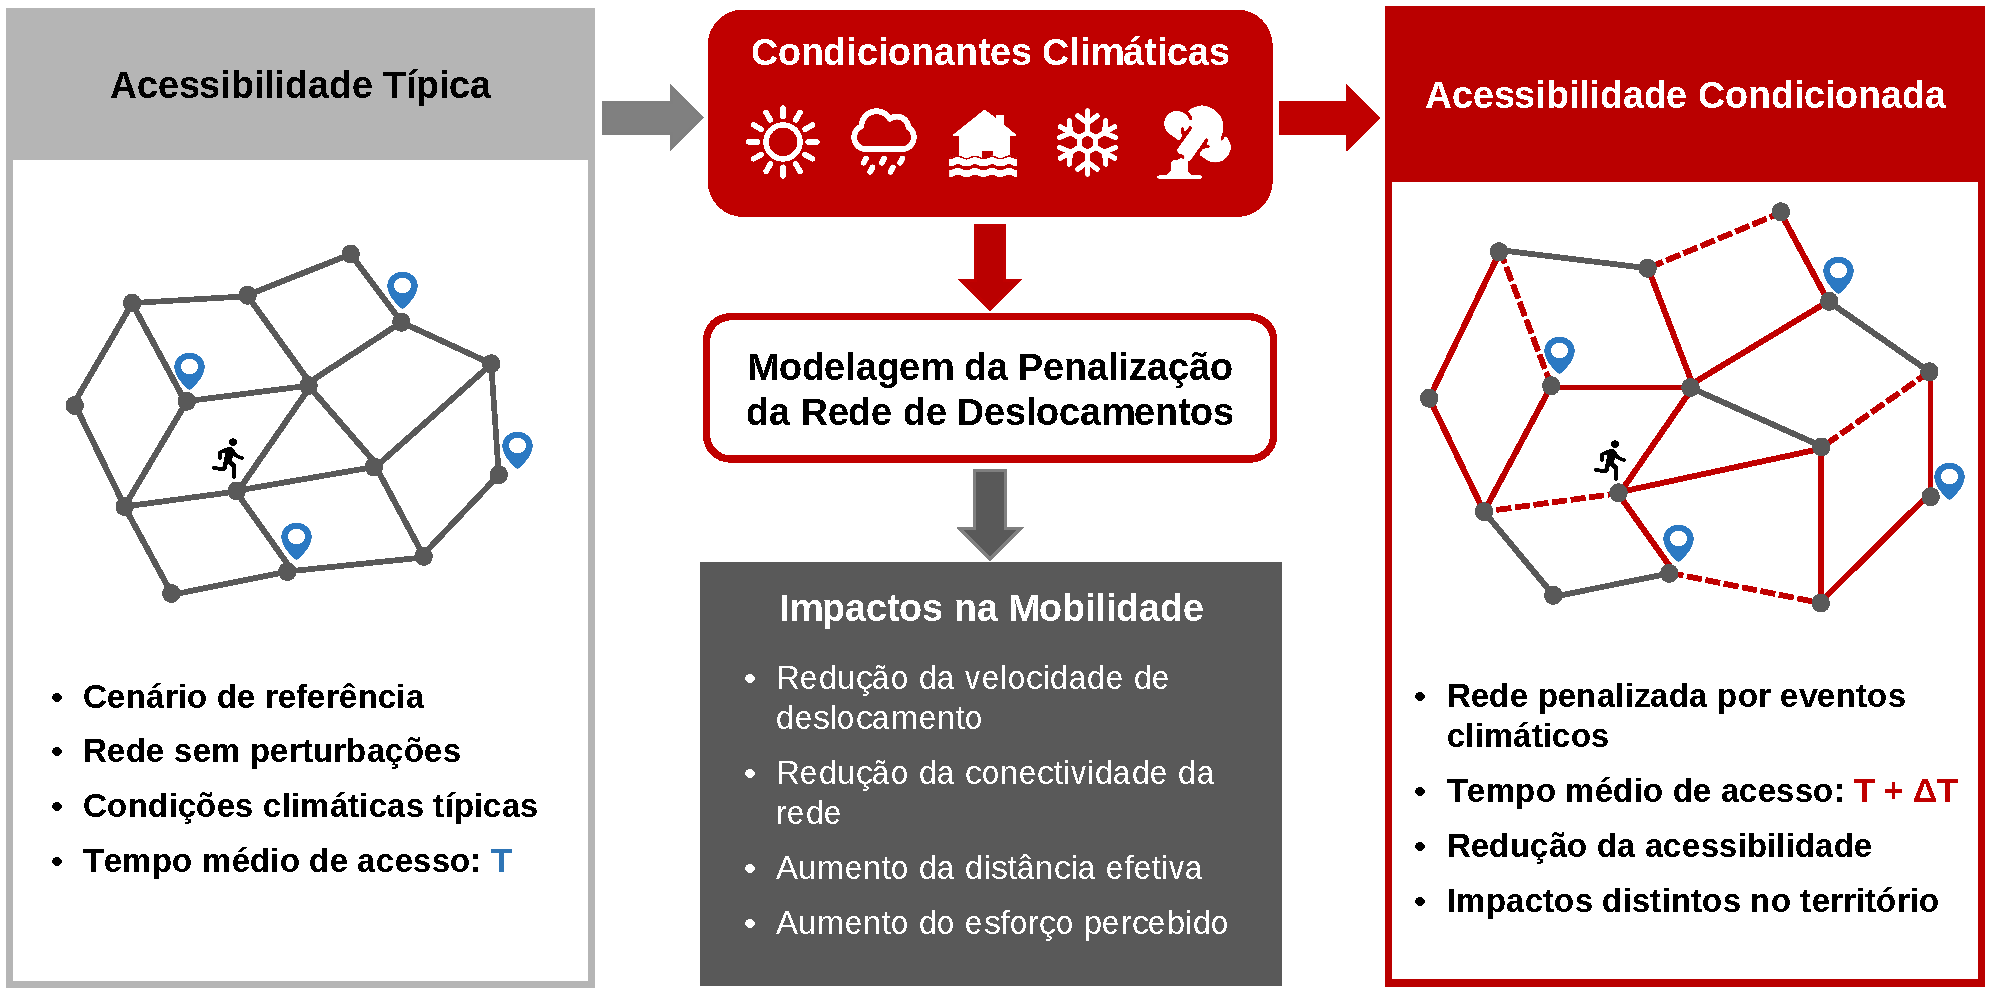
\includegraphics[width=1\textwidth]{figs/framework.pdf}
  \caption{Fluxo de modelagem dos cenários de acessibilidade. À esquerda, a rede no cenário típico, com seus custos originais de deslocamento. Ao centro, o mecanismo de penalização, que utiliza dados ambientais para penalizar a infraestrutura de mobilidade. À direita, o cenário condicionado, no qual o aumento do comprimento das arestas representa visualmente o acréscimo no tempo ou custo de deslocamento provocado pela perturbação.}
  \label{fig:framework}
\end{figure}

% O restante da Seção está estruturado da seguinte forma: a Subseção \ref{subsec:composition} apresenta o processo de coleta, pré-processamento e integração dos dados utilizados na modelagem do território urbano; a Subseção \ref{subsec:processing} descreve o método de cálculo dos indicadores de mobilidade e acessibilidade em diferentes cenários; a Subseção \ref{subsec:comparative} detalha os procedimentos para comparação entre os cenários ideal, típico e condicionado; a Subseção \ref{subsec:socioeconomical} expõe a integração de dados socioeconômicos, permitindo análises de desigualdades de acessibilidade; e, por fim, a Subseção \ref{subsec:case} explica os dados e ferramentas que serão utilizados no estudo de caso para aplicação da metodologia.

\subsection{Modelagem Territorial}
\label{subsec:territorial_modelling}

A modelagem do território urbano consiste na coleta, pré-processamento e integração de cinco camadas de dados espaciais que servem de base para a análise da acessibilidade:

\paragraph{1. Malha de análise:} Uma grade espacial regular que define a unidade mínima de estudo. A resolução da malha é ajustada ao modo de transporte e ao contexto local. O centroide de cada célula funciona como a origem teórica dos deslocamentos, servindo de base para o cálculo e a agregação dos indicadores.

\paragraph{2. Pontos de Interesse (POIs):} Representam os destinos dos deslocamentos. São coordenadas que indicam a localização dos serviços cotidianos da população, organizados em categorias (como saúde, educação e transporte). A seleção depende da disponibilidade de bases de dados locais, sejam oficiais ou colaborativas (crowdsourced).

\paragraph{3. Rede viária:} A infraestrutura de mobilidade é estruturada como um grafo espacial. Os vértices representam os cruzamentos e as arestas representam os segmentos de via, cujo peso base inicial corresponde à distância percorrida. Para possibilitar o cálculo de rotas reais, o centroide de cada célula da malha de análise é vinculado ao vértice mais próximo da rede.

\paragraph{4. Condicionantes ambientais:} Camadas espaciais, que podem ser contínuas (como imagens \textit{raster}) ou discretas (polígonos vetoriais), mapeando os fenômenos climáticos ou ambientais avaliados. Esses dados são sobrepostos à rede viária para reajustar o custo de deslocamento das arestas afetadas no cenário perturbado.

\paragraph{5. Dados Demográficos e Socioeconômicos:} Informações que caracterizam a população residente, como densidade demográfica, renda e escolaridade, oriundas de censos oficiais. Como esses dados são disponibilizados em unidades administrativas irregulares (como setores censitários), aplica-se um procedimento de compatibilização espacial para transferir o perfil socioeconômico para as células da malha regular de análise.

\subsection{Cenários e Perturbações}
\label{subsec:scenarios}

Nesta etapa, a rede de deslocamentos é avaliada em dois estados distintos: (1) Cenário Típico, que reflete as condições normais de mobilidade; e (2) Cenário Condicionado, no qual os custos da rede são alterados por variáveis ambientais.

No \textbf{Cenário Típico}, o peso de cada aresta do grafo ($W_{base}$) corresponde estritamente ao comprimento real do trecho da via. O tempo de percurso em condições normais é obtido dividindo-se essa distância pela velocidade média de deslocamento definida para o modo de transporte analisado.

No \textbf{Cenário Condicionado}, os custos de deslocamento são recalculados por meio de uma função de penalização. Esta função cruza a malha viária com as camadas de condicionantes ambientais ($C$), gerando um peso penalizado ($W_{condicionado}$) para cada aresta, estruturado na forma $W_{condicionado} = f(W_{base}, C)$. A aplicação geométrica dessa função varia conforme a natureza do dado ambiental:

\begin{itemize}
    \item \textbf{Dados contínuos} (ex.: \textit{rasters} de temperatura): O algoritmo extrai a média dos valores dos pixels que se sobrepõem geograficamente à aresta. Esse valor atua como um penalizador contínuo, aumentando o tempo de percurso proporcionalmente à severidade da condição ambiental ao longo daquele trecho.
    
    \item \textbf{Dados discretos} (ex.: polígonos de alagamento ou barreiras físicas): O algoritmo utiliza operações de interseção vetorial. A função pode aplicar multiplicadores severos ou atribuir peso infinito aos trechos interceptados, simulando interdições totais que forçam o roteamento a buscar caminhos alternativos. Essa mesma lógica de interseção pode ser usada de forma inversa, reduzindo pesos para simular áreas favoráveis (como vias arborizadas).
\end{itemize}

A forma matemática da função de penalização $f$ (linear, exponencial, limiar de corte) é um parâmetro ajustável. A escolha e calibração desses parâmetros devem considerar dados ou estudos do contexto local, já que a influência de variáveis ambientais sobre a velocidade e o esforço para caminhar varia conforme o clima, a cultura e as características urbanas. Evidências recentes mostram que fatores como temperatura, clima e condições viárias alteram significativamente o padrão e a velocidade da caminhada \cite{LIANG2020106811,Obuchi2021}. Por isso, recomenda-se que o aplicador utilize valores observados localmente ou reportados na literatura para definir as funções de penalização e os parâmetros do modelo.

Por fim, com os grafos dos dois cenários estruturados, um algoritmo de caminho de menor custo é executado para calcular as matrizes de tempo de viagem. A partir desses tempos, computam-se os indicadores apresentados na Seção \ref{subsubsec:indicadores}: o PTh de cada unidade territorial, o índice G (desigualdade) e o F15 (fração da população atendida) para ambos os cenários.

\subsection{Análise Comparativa}
\label{subsec:comparative}

Nesta etapa, quantificam-se as perdas de acessibilidade comparando diretamente os indicadores do cenário típico com os do cenário condicionado. O objetivo é mensurar a degradação da mobilidade imposta pelos fatores ambientais e identificar pontos críticos onde a dificuldade de circulação provoca maior isolamento.

Essa comparação é estruturada em três procedimentos analíticos principais:

\begin{itemize}
    \item \textbf{Variação relativa:} Cálculo das diferenças absolutas e percentuais dos tempos de deslocamento e dos níveis de acesso entre os dois cenários, evidenciando a magnitude da perda para cada unidade da malha.
    \item \textbf{Validação estatística:} Aplicação de testes de hipótese para confirmar a significância das alterações nos tempos de acesso provocadas pela perturbação ambiental em relação à rede original.
    \item \textbf{Mapeamento espacial:} Uso de métodos de associação local ou clusterização sobre as diferenças de tempo. Isso permite identificar, agrupar e mapear as manchas de degradação, revelando geograficamente as áreas mais penalizadas da cidade.
\end{itemize}

\subsection{Análise de Desigualdade Socioeconômica}
\label{subsec:socioeconomical}

Nesta etapa, as perdas de acessibilidade são analisadas em conjunto com os atributos socioeconômicos da população, com o objetivo de identificar padrões de vulnerabilidade associados às perturbações ambientais.

Cada célula da malha de análise, já associada aos dados sociodemográficos por compatibilização espacial, é tratada como unidade de observação. Para cada célula, consideram-se tanto os indicadores de acessibilidade no cenário típico ($PT_h$) quanto as variações induzidas pela perturbação ($\Delta PT_h$).

Inicialmente, aplica-se um modelo de regressão linear, no qual $PT_h$ e $\Delta PT_h$ são utilizados como variáveis dependentes em especificações distintas. As variáveis independentes incluem renda média, nível de escolaridade, densidade populacional e demais indicadores disponíveis. Esse procedimento permite estimar a associação entre características socioeconômicas e níveis de acessibilidade, bem como sua variação sob condições adversas.

Complementarmente, realiza-se uma análise de agrupamento socio-espacial, na qual as células são agrupadas considerando simultaneamente sua proximidade geográfica e a similaridade em termos de atributos socioeconômicos e indicadores de acessibilidade. Esse procedimento resulta em regiões adjacentes e internamente homogêneas, permitindo identificar padrões territoriais de desigualdade e vulnerabilidade de forma integrada.

% https://geoportal.sgb.gov.br/geosgb/
\subsection{Estudo de Caso}
\label{subsec:case_study}

Para demonstrar a viabilidade da metodologia proposta, o modelo será aplicado em duas capitais brasileiras: Curitiba (PR) e Porto Alegre (RS). A escolha desses municípios permite testar os dois comportamentos da função de penalização definidos na Seção \ref{subsec:scenarios}: o impacto de perturbações ambientais contínuas (temperatura de superfície) e discretas (áreas de risco geológico).

Para garantir a reprodutibilidade da pesquisa, os experimentos priorizam a utilização de dados abertos e bases governamentais oficiais.

\subsubsection{Curitiba: Degradação por Variável Contínua (Clima)}
O experimento em Curitiba avaliará como o desconforto térmico afeta a mobilidade ativa. Neste cenário, a temperatura de superfície atuará como um penalizador contínuo do esforço de deslocamento, aumentando o peso das arestas mais expostas ao calor. Os dados utilizados compreendem:

\begin{itemize}
    \item \textbf{Malha de deslocamento:} Rede viária extraída do OpenStreetMap (OSM), filtrada para infraestrutura caminhável.
    \item \textbf{Pontos de Interesse (POIs):} Coletados via OSM, complementados e validados por bases de alvarás municipais da Prefeitura de Curitiba, categorizados por tipos de serviço.
    \item \textbf{Condicionante ambiental:} Imagens de satélite (\textit{rasters}) do produto \textit{Surface Temperature} obtidas via Earth Explorer (Landsat 8 e 9, sensor TIRS - banda ST\_TRAD).
\end{itemize}

\subsubsection{Porto Alegre: Degradação por Variável Discreta (Risco Físico)}
O experimento em Porto Alegre analisará o impacto de áreas de risco geotécnico e físico sobre a acessibilidade urbana. Como condicionantes ambientais, serão utilizadas camadas vetoriais (polígonos) de \textit{Áreas com Risco a Movimentos de Massa} e \textit{Áreas de Risco Geológico}, ambas disponíveis no portal GeoPOA\footnote{\url{https://gis-smamus.portoalegre.rs.gov.br/dmweb-2-0/}} e resultantes de mapeamento realizado pelo Serviço Geológico do Brasil (SCG/CPRM). Essas áreas atuam como variáveis discretas, simulando barreiras que interrompem ou penalizam rotas afetadas por riscos. Os dados considerados para o experimento são:

\begin{itemize}
    \item \textbf{Malha de deslocamento:} Rede viária extraída do OpenStreetMap (OSM);
    \item \textbf{Pontos de Interesse (POIs):} Serviços e instalações mapeados integralmente a partir do OSM;
    \item \textbf{Condicionantes ambientais:} Polígonos das \textit{Áreas com Risco a Movimentos de Massa} e \textit{Áreas de Risco Geológico} proveniente do GeoPOA (origem: SCG/CPRM).
\end{itemize}

Por fim, para a análise de desigualdade socioeconômica em ambos os municípios, as malhas territoriais serão enriquecidas com dados do Censo Demográfico do IBGE (Instituto Brasileiro de Geografia e Estatística), permitindo o cruzamento das perdas de acessibilidade com variáveis de renda, infraestrutura domiciliar e vulnerabilidade social.

\subsection{Limitações}
\label{subsec:limitations}

A calibração dos efeitos ambientais no modelo é limitada pela disponibilidade e qualidade dos dados ou por falta de estudos específicos. Por isso, os valores de indicadores como o PTh podem não representar tempos absolutos reais, sendo mais adequados para análises comparativas entre diferentes regiões do que para estimativas precisas de tempo. Dessa forma, o modelo cumpre melhor o papel de identificar padrões de desigualdade e vulnerabilidade territorial diante de perturbações ambientais do que de quantificar o tempo exato de acesso.

Além disso, há limitações relacionadas ao comportamento dos indivíduos. Em situações extremas, as pessoas podem optar por não se deslocar ou escolher modos de transporte diferentes da mobilidade ativa. O modelo pressupõe a manutenção do deslocamento a pé mesmo sob condições adversas, o que pode não refletir a realidade observada. Assim, os resultados simulam apenas o impacto potencial das perturbações na acessibilidade da rede, não substituindo análises que considerem efetivamente as escolhas modais dos usuários. Ressalta-se, ainda, que a metodologia pode ser adaptada para outros modos de transporte, mediante ajustes nos parâmetros de velocidade e custo.

Ainda, os indicadores calculados refletem apenas o potencial de acesso espacial e o esforço exigido para atingir determinados destinos, sem considerar fatores como a qualidade, capacidade, funcionamento ou atratividade dos serviços presentes nos POIs. Além disso, esses indicadores não capturam obstáculos subjetivos, como percepção de segurança, conforto ou preferência individual de rotas. Por isso, apesar de úteis para análise territorial comparativa, os resultados não devem ser interpretados como medida direta da experiência do usuário ou garantia de acesso efetivo aos serviços analisados.







% \section{Resultados e Discussões}
\label{sec:results}

Os experimentos desenvolvidos neste trabalho têm o intuito de verificar como variáveis socioeconômicas podem influenciar os tempos de acesso a pé aos pontos de interesse urbanos.

\subsection{Experimento 1 - Análise de Regressão}

O Experimento 1 resultou em um modelo de regressão linear com coeficiente de determinação (R²) de 0,73. Dentre as variáveis analisadas, 30 demonstraram efeitos estatisticamente significativos ($p < 0,005$). A Tabela \ref{tab:variaveis} (Apêndice A) detalha essas variáveis, incluindo seus nomes e descrições. A Figura \ref{fig:coef} apresenta os coeficientes e seus intervalos de confiança de 95\%, ordenados por magnitude de efeito. É importante destacar que as variáveis não foram padronizadas neste experimento. Portanto, embora a magnitude dos coeficientes não permita comparação direta sobre a influência relativa entre as variáveis, a direção do efeito (positiva ou negativa) mantém-se como um resultado relevante para a interpretação.

\begin{figure}[ht]
  \centering
  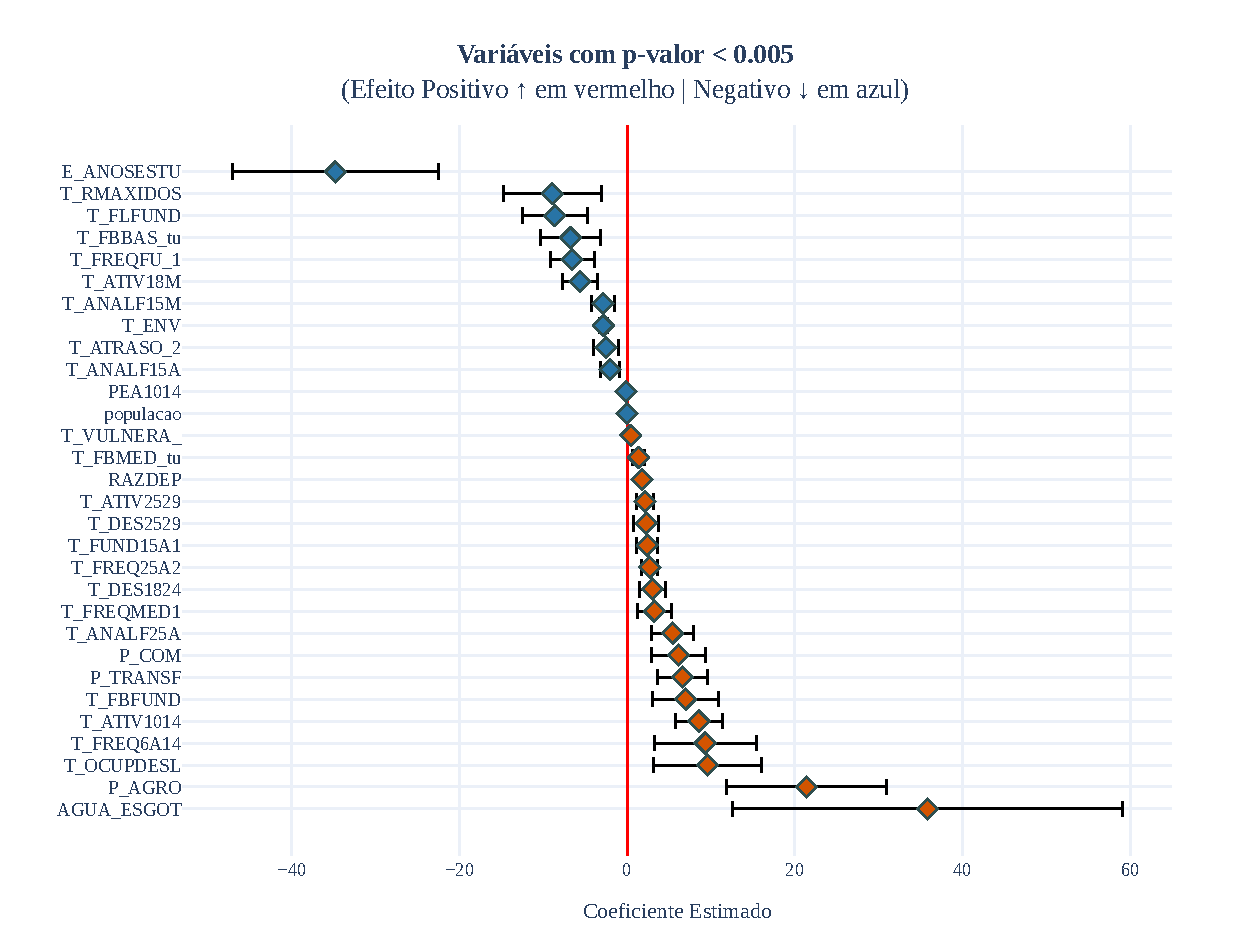
\includegraphics[width=0.8\textwidth]{figs/coeficientes.pdf} % Ou .svg/.eps
  \caption{Efeito das variáveis no tempo de acesso (IC95\%).}
  \label{fig:coef}
\end{figure}

O modelo identificou doze variáveis com associação negativa com o tempo de acesso, indicando que maiores valores nestes indicadores correspondem a menores tempos de deslocamento. Sete entre as doze variáveis com efeito negativo sugerem que áreas com melhores indicadores educacionais e maior participação econômica tendem a apresentar melhor acessibilidade urbana, sendo elas: (1) expectativa de anos de estudo aos 18 anos, (2) taxa de frequência líquida ao ensino fundamental, (3) taxa de frequência bruta ao ensino básico, (4) percentual da população de 15 a 17 anos frequentando o ensino fundamental, (5) taxa de pessoas maiores de 18 anos economicamente ativas, (6) taxa de envelhecimento e (7) tamanho da população.

O modelo também identificou cinco variáveis com indicadores sociais adversos que, paradoxalmente, apresentaram associação negativa com o tempo de acesso: (i) percentual de pessoas em domicílios vulneráveis à pobreza e dependentes de idosos, (ii) taxa de analfabetismo na população com mais de 15 anos, (iii) percentual de estudantes de 6 a 17 anos com atraso idade-série maior que 2 anos, (iv) taxa de analfabetismo na população de 15 a 17 anos, e (v) população economicamente ativa de 10 a 14 anos. Esses resultados aparentemente contraintuitivos podem sugerir tanto um artefato espacial (com a concentração dessas condições em áreas próximas a regiões centrais mais servidas por \ac{pois}) quanto a necessidade de investigar outros mecanismos subjacentes não capturados pelo modelo atual.

Dezoito variáveis apresentaram associação positiva com o tempo de acesso, sendo as mais intuitivas aquelas relacionadas a vulnerabilidades estruturais: (a) indicadores de inatividade juvenil, (b) razão de dependência demográfica (proporção de pessoas economicamente dependentes – crianças e idosos – em relação à população em idade ativa – entre 15 e 64 anos), (c) analfabetismo em adultos jovens (25-29 anos), e (d) concentração ocupacional em setores primários e comercio e taxa de desemprego de pessoas de 25 a 29 anos. Complementando esse perfil, destacam-se (e) trabalho infantil (atividade 10-14 anos) e (f) precariedade domiciliar (infraestrutura sanitária inadequada e longos tempos de deslocamento). Esses resultados confirmam expectativas teóricas sobre a penalidade de acessibilidade temporal em territórios com inserção econômica precária. 

Dentre essas dezoito variáveis, cinco apresentaram associações positivas que contrariam hipóteses iniciais: (g) taxa de frequência bruta ao ensino médio regular, (h) percentual de jovens de 18-24 anos no ensino médio regular, (i) taxa de frequência bruta ao ensino fundamental regular, (j) taxa de atendimento escolar (6-14 anos) e (k) taxa de atividade econômica (25-29 anos). Esses resultados inesperados destacam a complexidade da relação entre indicadores socioeconômicos e acessibilidade temporal urbana, revelando tanto limitações do modelo linear quanto mecanismos subjacentes não capturados pela análise. Esses resultados podem ser melhor compreendidos através da análise de clusterização desenvolvida no Experimento 2 que examina como a combinação dessas variáveis se distribui no território e compara as médias dos tempos de acesso entre os clusters identificados.

\subsection{Experimento 2 - Análise de Clusterização}

A clusterização foi realizada nas duas primeiras componentes principais (PC1 e PC2), que juntas explicam 63,2\% da variância total. Para interpretar os clusters, examinamos as cargas (loadings) das variáveis originais nas componentes PC1 e PC2, como mostra a Figura \ref{fig:loadings}. A primeira componente (PC1), responsável por 44,8\% da variância, está fortemente correlacionada com variáveis socioeconômicas, como renda e escolaridade, consolidando-se como um eixo de estratificação social. Já a segunda componente (PC2), que explica 18,4\% da variância, associa-se predominantemente ao tempo de acesso a \ac{pois} em diferentes categorias (variáveis A1 – A64), revelando um eixo de acessibilidade temporal.

\begin{figure}[ht]
  \centering
  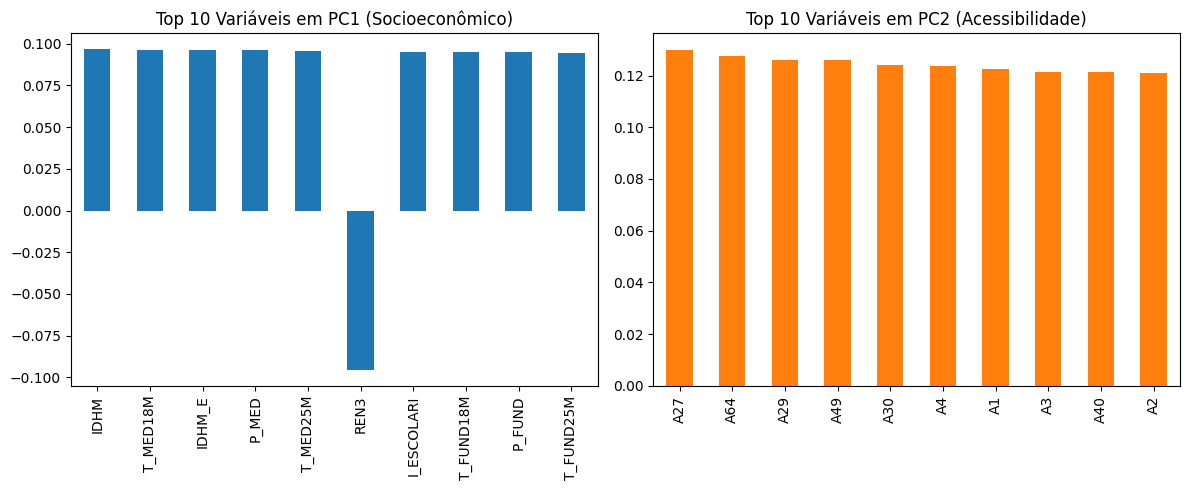
\includegraphics[width=\textwidth]{figs/top_pc_vars.png}
  \caption{Cargas das 10 variáveis mais influentes nas componentes principais PC1 e PC2.}
  \label{fig:loadings}
\end{figure}

O método do cotovelo indicou k=4 como um número adequado de clusters, cuja distribuição espacial é apresentada na Figura \ref{fig:clusters}. A análise revela quatro padrões territoriais distintos: o \textbf{Cluster 1 (Alto)} concentra-se em regiões centrais e bairros planejados, exibindo altas cargas positivas em PC1; o \textbf{Cluster 2 (Médio)} ocupa áreas adjacentes ao centro, com valores intermediários em ambas as componentes; o \textbf{Cluster 3 (Baixo)} caracteriza periferias consolidadas, marcadas por baixos valores em PC1 e PC2; enquanto o \textbf{Cluster 4 (Rural)} identifica periferias distantes de baixa densidade populacional, com cargas moderadamente baixas em PC1 e negativas em PC2, sugerindo vulnerabilidades socioespaciais moderadas e elevados tempos de acesso.

\begin{figure}[!htbp]
  \centering
  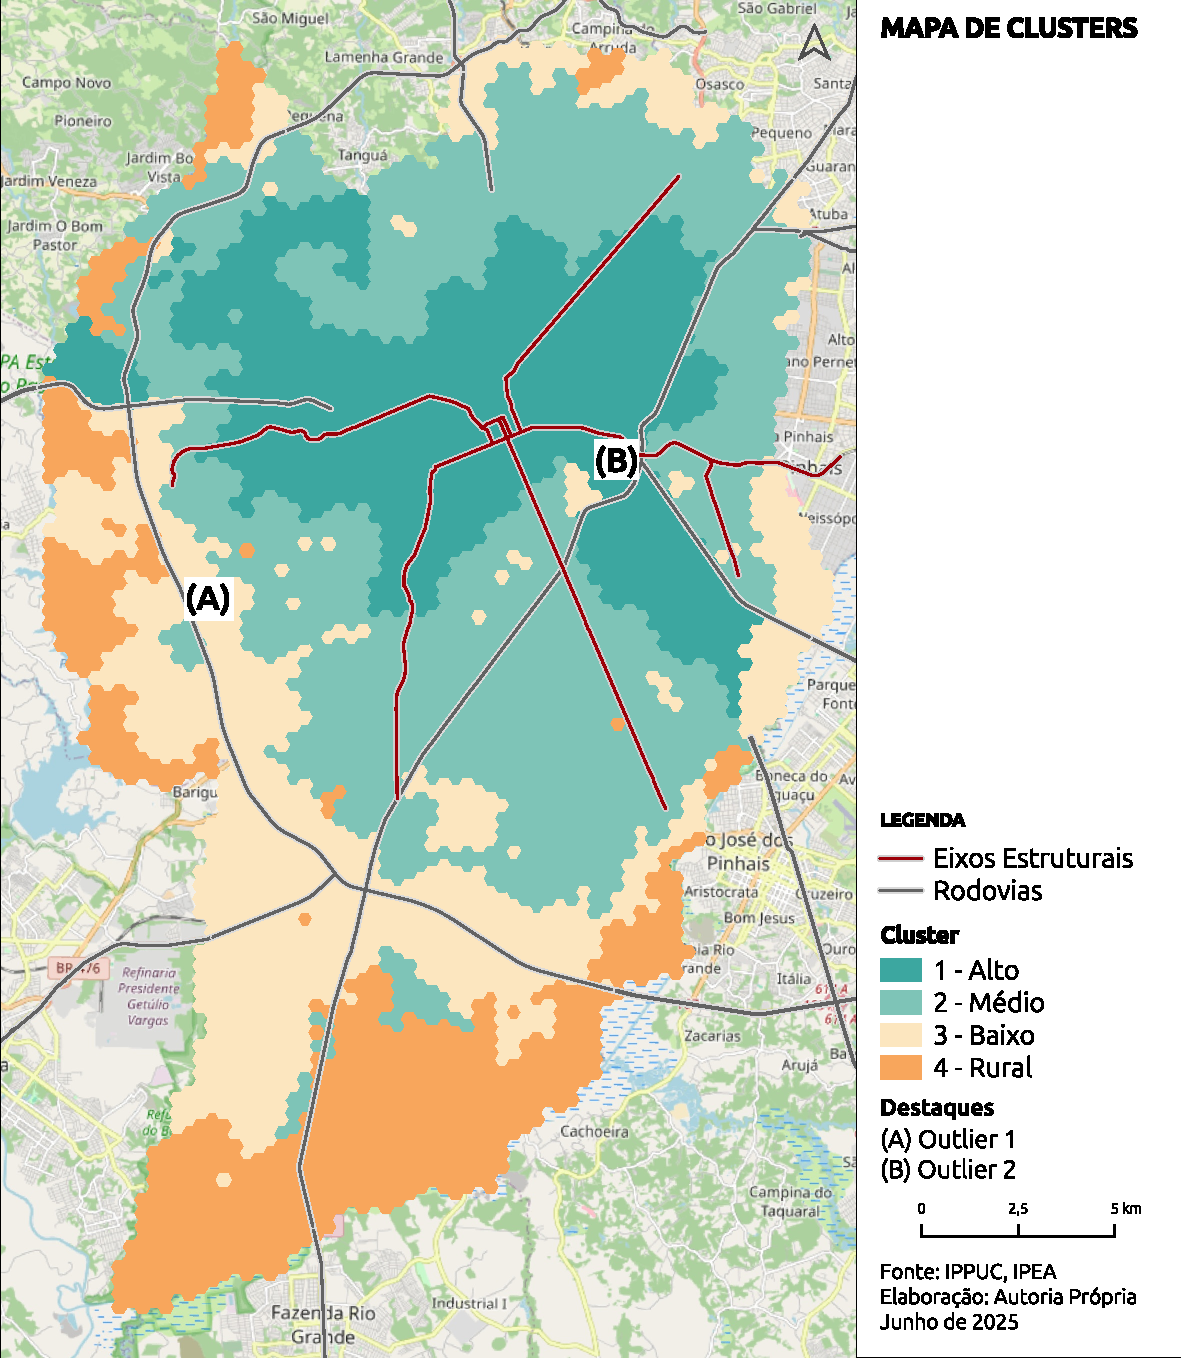
\includegraphics[width=0.6\textwidth]{figs/mapa_clusters_v2.pdf}
  \caption{Distribuição espacial dos clusters.}
  \label{fig:clusters}
\end{figure}

Os boxplots presentes na Figura \ref{fig:boxplots} revelam padrões claros de desigualdade entre os clusters. Para variáveis associadas a condições socioeconômicas favoráveis, como anos de estudo (E\_ANOSESTU) e frequência líquida ao ensino médio (T\_FLMED), observa-se uma gradativa redução das medianas e ampliação da dispersão à medida que se avança do Cluster 1 para o Cluster 3. O Cluster 1 apresenta distribuições concentradas em valores altos (ex.: mediana ao redor de 12,5 anos de estudo), enquanto o Cluster 3 exibe maior variabilidade e valores significativamente inferiores (ex.: mediana ao redor de 11,2 anos), refletindo disparidades educacionais. Já variáveis como T\_NESTUDA\_ (taxa de pessoas de 15 a 24 anos que não estudam e não trabalham e são vulneráveis a pobreza) e AGUA\_ESGOT (acesso inadequado a água e esgoto) seguem o padrão inverso, com piores indicadores no Clusters 3, corroborando a associação entre privação material e exclusão de serviços básicos.

A dimensão espacial também é evidente. O tempo de acesso a serviços (tempo\_acesso) é sistematicamente maior nos clusters periféricos (3 e 4), indicando que parte da população enfrenta deslocamentos excessivos. Em contraste, a expectativa de vida (ESPVIDA) tem queda abrupta para o Cluster 3 e o percentual de pessoas em domicílios com paredes que não sejam de alvenaria ou madeira aparelhada (PAREDE) tem aumento neste mesmo grupo, sugerindo que a combinação de baixos indicadores socioeconômicos e acessibilidade limitada potencializa vulnerabilidades.

A análise revela dois outliers: (A) uma vila residencial inserida em zona industrial, com uma densidade de \ac{pois} maior que a observado no Cluster 3, incluindo equipamentos públicos de qualidade, e indicadores de educação e infraestrutura superiores aos do entorno imediato; e (B) um assentamento precário em região central, cuja desorganização urbana (falta de pavimentação, ausência de equipamentos públicos) neutraliza completamente as vantagens da localização, aprofundando a exclusão socioespacial.

%\clearpage

\begin{figure}[!htbp]
{
  \centering
  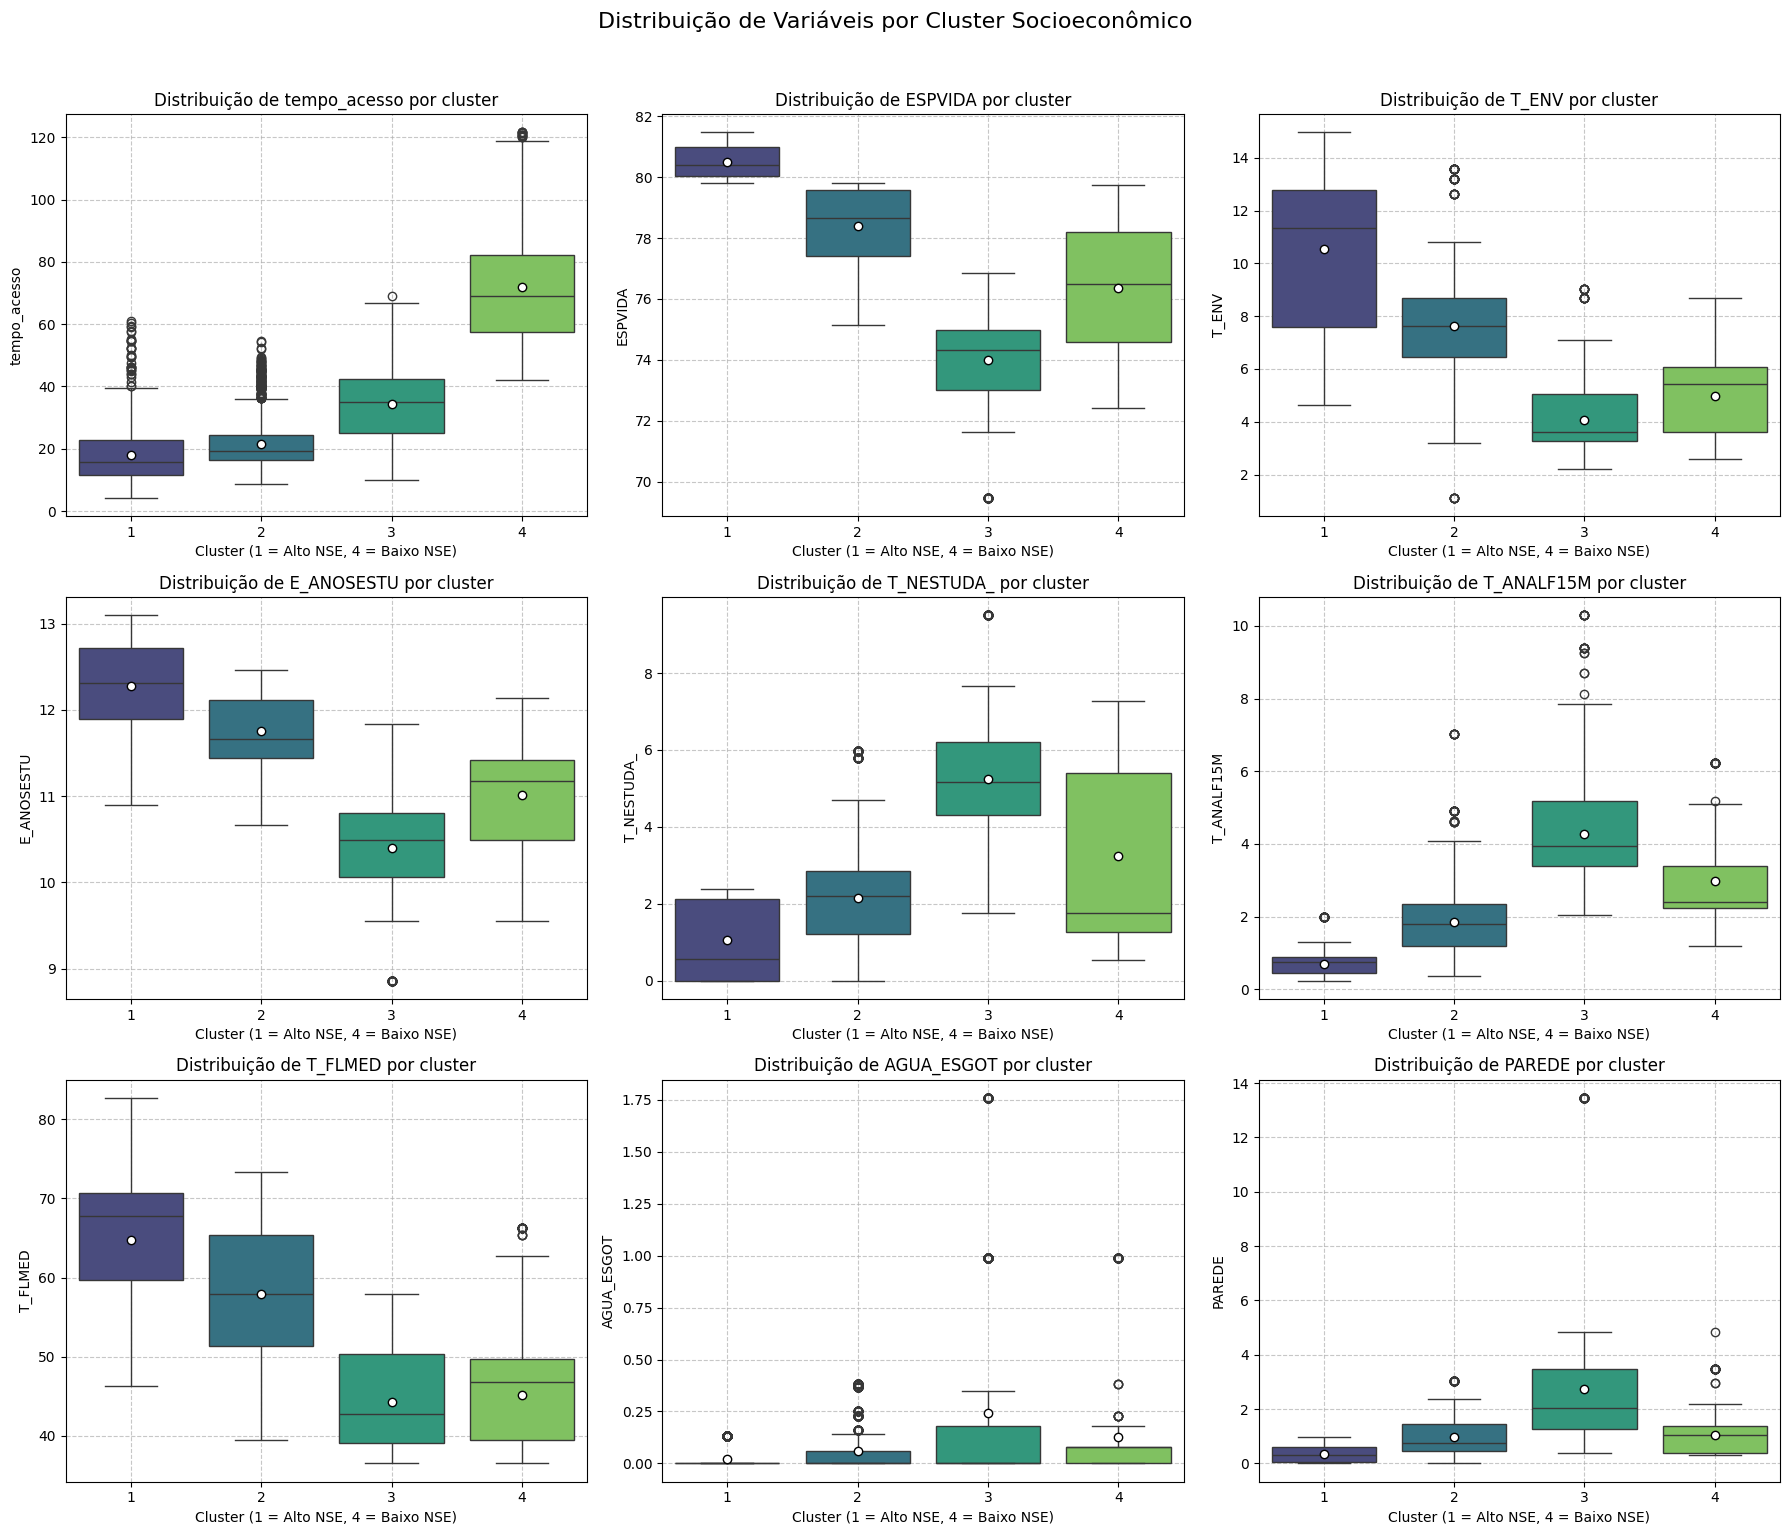
\includegraphics[width=\textwidth]{figs/cluster_boxplots.png}
  \caption{Distribuição de variáveis por cluster socioeconômico}
  \label{fig:boxplots}
}
\end{figure}
% \section{Considerações Finais}
\label{sec:considerations}

Este estudo combinou análise de regressão e clusterização espacial para investigar como desigualdades socioeconômicas moldam os tempos de acesso a pé em Curitiba. Foi demonstrado que variáveis socioeconômicas como aquelas associadas à escolaridade e empregabilidade explicam variações nos tempos de acesso (Experimento 1), enquanto que a análise de clusterização (Experimento 2) caracterizou grupos intraurbanos heterogêneos levando em consideração aspectos socioeconômicos e tempos médios.

Os resultados contraintuitivos sobre o efeito das variáveis socioeconômicas (g-k) nos tempos de acesso sugerem que a relação entre fatores socioeconômicos e tempo de acesso não é direta. Essa complexidade fica evidente através da análise de clusters, que revela padrões locais que ajudam a explicar essas relações contraditórias. Um exemplo disso são áreas com alta densidade de \ac{pois} que, apesar disso, não apresentam desenvolvimento socioeconômico elevado, indicando que condições socioeconômicas não são os únicos determinantes dos tempos de acesso. No entanto, é importante ressaltar que este estudo não avaliou a qualidade ou a efetividade desses \ac{pois}, o que pode ser determinante para compreender as disparidades observadas.

O estudo não capturou dinâmicas temporais (ex.: variações horárias na oferta de serviços) e focou exclusivamente na acessibilidade temporal a pé, deixando de considerar critérios qualitativos como capacidade de atendimento, condições físicas ou barreiras morfológicas – fatores que influenciam diretamente a efetividade do acesso. Além disso, outros modos de mobilidade, como bicicleta ou transporte coletivo, não foram incluídos na análise, uma limitação a ser explorada em trabalhos futuros.

Parte da redação deste artigo e dos códigos computacionais utilizados foram desenvolvidos com assistência de ferramentas de IA generativa, empregadas para: (i) aprimorar a clareza textual, (ii) sugerir métodos de validação estatística, e (iii) otimizar a visualização de dados. Todo conteúdo gerado foi rigorosamente validado e adaptado, garantindo precisão conceitual e seguindo princípios éticos de pesquisa acadêmica.

\section{Agradecimentos}
\label{sec:acknoledgments}

Ao Ippuc pela disponibilização dos dados de acessos intraurbanos. Ao SocialNet/FAPESP (2023/00148-0) e CNPq (444724/2024-9, 441444/2023-7) pelo apoio. Aos revisores e colegas pelas contribuições.

\section{Introdução}

A mobilidade ativa, isto é, a mobilidade cujos deslocamentos são realizados a pé, de bicicleta ou por algum outro meio que não envolva a utilização de veículos individuais motorizados, pode contribuir na mitigação de impactos climáticos. Segundo \cite{BRAND2021102764}, cerca de 70\% das emissões de ciclo de vida de CO2 por pessoa de atividades relacionadas a mobilidade urbana são geradas por carros frente a apenas 1\% das emissões geradas por bicicleta. Os autores ainda estimam que cada deslocamento de carro evitado reduz em 62\% as emissões por indivíduo.

Em resposta à urgência climática e em busca da criação de políticas de descarbonização, diversos modelos de planejamento urbano vêm sendo desenvolvidos. Um modelo de destaque, atualmente em implantação em importantes cidades como Paris e Barcelona, é o modelo de cidade de 15 minutos \cite{Allam2022-yx}. Neste modelo, a cidade é organizada de forma que os principais serviços utilizados no dia a dia da população possam ser acessados através de deslocamentos de curta distância, priorizando a mobilidade ativa.

Contudo, a viabilidade de modelos como a cidade de 15 minutos depende fundamentalmente de como a rede de deslocamentos se comporta sob condições reais de operação. Trabalhos anteriores demonstraram que a acessibilidade urbana não é uniforme: desigualdades socioeconômicas moldam fortemente quem tem acesso a quais serviços e em qual tempo \cite{sbbd_estendido}. Além disso, eventos climáticos extremos (inundações, chuvas intensas, escorregamentos) degradam a infraestrutura de mobilidade, interrompendo ou dificultando trechos da rede viária e tornando certos deslocamentos inviáveis ou significativamente mais custosos. Essas perturbações não afetam a população de forma uniforme: áreas mais vulneráveis frequentemente apresentam menor resiliência à degradação da rede e populações com menor capacidade de adaptação sofrem maiores impactos.

Este trabalho avalia como perturbações climáticas modificam a acessibilidade urbana e como esses impactos se distribuem desigualmente no espaço e entre perfis socioeconômicos, propondo uma abordagem metodológica que integra modelagem de redes de deslocamento com análise socioeconômica e compara cenários típicos (sem perturbação) e cenários condicionados por variáveis ambientais. Com isso, contribui para a compreensão de como garantir equidade na acessibilidade urbana sob cenários de perturbação ambiental.
\section{Fundamentos e Trabalhos Relacionados}
Esta seção descreve os fundamentos teóricos e discute trabalhos
relacionados.

\subsection{Acessibilidade Urbana}

Em estudos urbanos e de transportes, acessibilidade urbana descreve a facilidade em alcançar oportunidades (serviços, empregos, equipamentos e atividades) a partir de um local de origem. Diferente de mobilidade (movimento observado), acessibilidade é uma propriedade estrutural do sistema urbano: depende de onde as oportunidades estão, de como a rede conecta origens e destinos e de quais impedâncias (custos) são impostas ao deslocamento~\cite{Handy1997Measuring}. Assim, ela é frequentemente tratada como uma medida de potencial de acesso, e não como uma medida direta de viagens realizadas.

Formalizando o problema matematicamente e espacialmente, o território pode ser representado por um conjunto de origens $O$ (por exemplo, células territoriais, centróides de setores, quadras ou pontos de residência) e um conjunto de destinos $D$ (pontos de interesse, POIs). Define-se então uma função de custo $c(o,d)$ que associa a cada par $(o,d)$ o custo mínimo de deslocamento entre $o \in O$ e $d \in D$~\cite{Miller1999Measuring}. Em aplicações baseadas em rede, esse custo é tipicamente obtido por algoritmos de caminho mínimo em um grafo de deslocamento (por exemplo, tempo de caminhada ou ciclismo), e serve de base para construir indicadores comparáveis entre diferentes áreas e cenários.

Embora frequentemente expresso como tempo ou distância, o custo $c(o,d)$ pode ser entendido de forma mais geral como uma impedância composta, incorporando fatores como conforto, segurança, esforço físico e confiabilidade do percurso~\cite{Puello2016Integration}. Esse ponto é particularmente importante para mobilidade ativa~\cite{Cook2022More} em curta distância, na qual a experiência do percurso e condições locais (declividade, travessias, qualidade de calçadas, exposição ao sol/chuva/vento, presença de alagamentos) podem alterar a viabilidade do deslocamento mesmo quando a geometria da rede permanece a mesma. Dessa forma, perturbações climáticas podem ser incorporadas ao problema como alterações no custo generalizado de deslocamento, e não apenas como bloqueios binários de segmentos.

Dentro das medidas de acessibilidade baseadas em localização, revisões como a de \cite{Geurs2004} indicam que é comum organizar os indicadores em famílias segundo seus pressupostos: (i) medidas de distância (ou custo mínimo), (ii) medidas cumulativas (ou de contorno) e (iii) medidas potenciais (ou gravitacionais). Essas famílias diferem na forma como tratam a escolha de destinos, a substituibilidade entre oportunidades e o papel do decaimento com a distância/tempo, mas compartilham a ideia central de que a acessibilidade é derivada de uma matriz de custos origem-destino.

As medidas mais simples são as métricas de distância, nas quais a acessibilidade de uma origem é representada pelo custo mínimo até a oportunidade mais próxima (por exemplo, o tempo até o comércio mais próximo). Esse indicador é intuitivo e útil quando se assume que usuários tendem a satisfazer a necessidade no destino mais fácil de alcançar; por outro lado, ele ignora a existência de múltiplas alternativas, não representa competição entre ofertas e pode ser instável quando pequenas mudanças na rede fazem com que mude também o POI mais próximo.

Quando a disponibilidade de múltiplas oportunidades está em jogo, usam-se medidas cumulativas (de contorno), que contam quantas oportunidades estão acessíveis dentro de um limiar de custo (por exemplo, número de POIs em até 15 minutos). Uma variação útil quando se deseja evitar a escolha de um limiar fixo --- e, ao mesmo tempo, manter a interpretação intuitiva --- é calcular a acessibilidade a partir do custo médio para acessar as $N$ oportunidades mais próximas, por categoria de serviço. Assim, a métrica passa a representar a "facilidade média" de alcançar um conjunto mínimo de alternativas relevantes, o que se alinha com deslocamentos de curta distância em que a população costuma ter um conjunto pequeno de opções efetivamente consideradas.

Apesar de sua clareza, métricas cumulativas e variantes por $N$ vizinhos carregam escolhas operacionais que afetam o resultado: o valor do limiar (quando existe), o valor de $N$, a sensibilidade a empates e a forma como oportunidades são ponderadas (todas iguais ou com pesos). Além disso, tais medidas tendem a tratar o custo como um corte abrupto (dentro/fora do conjunto acessível) ou como uma média simples, o que pode sub-representar mudanças graduais na atratividade de destinos à medida que o custo aumenta. Em cenários de perturbação climática, nos quais o custo pode se alterar de forma contínua e espacialmente desigual, torna-se útil empregar formulações que penalizem destinos mais distantes de modo progressivo, sem depender de um corte rígido.

Nas métricas potenciais (ou gravitacionais), a acessibilidade é calculada como a soma das oportunidades ponderadas por uma função de decaimento do custo, capturando a ideia de que destinos mais distantes contribuem menos para a acessibilidade do que destinos próximos. A formulação clássica, de \cite{Hansen1959}, expressa a acessibilidade de uma origem $o$ como
\begin{equation}
A(o) = \sum_{d \in D} W_d \, f\!\big(c(o,d)\big),
\end{equation}
onde $W_d$ representa a massa ou atratividade da oportunidade no destino $d$ (por exemplo, capacidade, tamanho ou um peso unitário) e $f\!\big(c(o,d)\big)$ é uma função decrescente que reduz a contribuição à medida que o custo aumenta. Na prática, não é necessário considerar todos os destinos: é comum restringir o conjunto a uma vizinhança relevante (por exemplo, os $N$ destinos mais próximos ou destinos dentro de uma janela de custo), preservando o princípio do decaimento e evitando que oportunidades muito distantes tenham influência indevida ou que o indicador fique computacionalmente pesado.

A função de decaimento $f(c)$ pode assumir diferentes formas (exponencial, potência, logística), e seus parâmetros controlam o quanto a acessibilidade cai com o aumento do custo. Conceitualmente, isso permite aproximar diferentes comportamentos de escolha e diferentes tolerâncias ao deslocamento, e operacionalmente, esses parâmetros podem ser calibrados a partir de literatura, dados observados ou análises de sensibilidade. Para mobilidade ativa em curta distância, funções com decaimento relativamente forte tendem a ser coerentes com a queda rápida na propensão a caminhar/pedalar conforme o custo aumenta, especialmente quando o custo incorpora desconforto ambiental.

No quadro conceitual mais amplo, a acessibilidade resulta da interação entre componentes de uso do solo (onde estão as oportunidades), transporte (rede e impedâncias), temporalidade (variações por horário/estação/evento) e características individuais (restrições e preferências). Este trabalho foca principalmente na componente de transporte/impedância ao comparar um cenário típico, em que os custos derivam da topologia e dos pesos usuais da rede, e um cenário condicionado por perturbações climáticas, no qual os pesos das arestas são penalizados por variáveis ambientais. Mantendo constantes (ou controladas) as oportunidades e a representação espacial das origens, a diferença entre os indicadores nos dois cenários passa a expressar a sensibilidade/robustez da acessibilidade frente a perturbações climáticas.

Diante dessas definições, diferentes métricas têm sido propostas para sintetizar e comparar o acesso às oportunidades no ambiente urbano. Entre elas, destacam-se indicadores que permitem descrever o nível de acessibilidade em cada área da cidade e avaliar a distribuição desse acesso entre a população.

\subsubsection{Indicadores de Acessibilidade em Curta Distância}
\label{subsubsec:indicadores}

Para calcular a acessibilidade urbana a serviços cotidianos, \cite{Bruno2024} utilizam um conjunto de indicadores territoriais e de desigualdade, baseados em uma malha espacial regular como unidade mínima de análise.

\paragraph{PTh (Proximity Time por unidade territorial):} Tempo médio necessário para 
alcançar os $k$ pontos de interesse mais próximos de uma categoria de serviço \ric{$i$}?, a partir 
de cada célula territorial:

\begin{equation}
    PTh_i = \frac{1}{k} \sum_{d \in D_k(i)} c(i,d),
\end{equation}

\noindent onde $D_k(i)$ é o conjunto dos $k$ POIs mais próximos e $c(i,d)$ é o tempo 
mínimo de deslocamento na rede. O parâmetro $k$ é ajustável conforme o contexto 
($k=1$ para saúde de emergência; $k=2$ ou $k=3$ para educação e comércio). Menores 
valores de PTh indicam maior acessibilidade. Calculado para cada célula, PTh organiza-se 
como uma camada espacial, revelando gradientes territoriais e padrões de concentração 
de oportunidades.

\paragraph{Índice G (desigualdade de acessibilidade):} Coeficiente de Gini que mede 
como a acessibilidade é distribuída entre territórios ou grupos socioeconômicos. 
Varia de 0 (igualdade perfeita) a 1 (desigualdade máxima). Valores mais altos indicam 
maior concentração de má acessibilidade em parcelas específicas da população. É 
particularmente útil para comparar como a distribuição de acessibilidade muda entre 
cenários, revelando se perturbações ambientais amplificam ou reduzem desigualdades.

\paragraph{F15 (Fração da população em zonas de 15 minutos):} Proporção da população
residente em células onde PTh $\leq$ 15 minutos:

\begin{equation}
    F15 = \frac{\sum_i p_i \cdot \mathbb{1}(PTh_i \leq 15)}{\sum_i p_i} \times 100\%,
\end{equation}

\noindent onde $\mathbb{1}(\cdot)$ é uma função indicadora e $p_i$ representa a população residente na unidade territorial $i$. Diferencia-se de PTh por 
ser binária (dentro ou fora do limiar) e é utilizada complementarmente para avaliar 
cobertura de população sob o modelo de cidade de 15 minutos.

\subsection{Grafos e Redes de Mobilidade}

Em termos de formalização e modelagem da acessibilidade, o custo mínimo $c(o,d)$ é geralmente obtido a partir de uma rede de deslocamento representada como um grafo ponderado $G=(V,E)$. Nessa representação, os vértices $V$ correspondem a pontos de decisão na malha viária (como interseções e nós topológicos), enquanto as arestas $E$ representam segmentos percorríveis (ruas, passagens e conexões). A cada aresta $e \in E$ associa-se um peso $w(e)$, que codifica o esforço necessário para atravessá-la.

Em muitos contextos, a rede pode ser tratada como não-direcionada, isto é, assumindo-se que o deslocamento ao longo de um segmento possui custo equivalente em ambos os sentidos. Contudo, há situações em que a impedância depende do sentido de percurso, o que torna adequada a representação por um grafo direcionado, permitindo custos distintos para cada orientação de uma mesma conexão (por exemplo, devido a declividade, escadas, travessias controladas ou restrições de circulação). Essa distinção é relevante porque altera o conjunto de caminhos viáveis considerados no cálculo de $c(o,d)$.

No caso de caminhadas, uma modelagem simples e amplamente utilizada define $w(e)$ como o tempo de percurso, estimado a partir do comprimento geométrico do segmento e de uma velocidade de caminhada assumida. Em formulações mais gerais, o peso pode ser interpretado como custo generalizado, incorporando penalidades adicionais relacionadas à qualidade do ambiente. Com isso, o custo entre uma origem $o$ e um destino $d$ é dado pelo custo do menor caminho na rede, isto é, pela soma mínima dos pesos ao longo de um caminho viável:
\begin{equation}
    c(o,d) = \min_{p} \sum_{e \in p} w(e),
\end{equation}
com $p \in \mathcal{P}(o,d)$, o conjunto de caminhos possíveis entre $o$ e $d$. Do ponto de vista algorítmico, esse valor pode ser calculado por métodos clássicos de caminhos mínimos, como o algoritmo de Dijkstra \cite{cormen01introduction}, ou variantes com heurística, como $A^*$, dependendo das propriedades do grafo e dos requisitos de desempenho da aplicação.

De forma geral, mudanças nas condições de deslocamento podem ser representadas na rede tanto como alterações contínuas de impedância quanto como restrições de circulação que tornam determinados segmentos indisponíveis. Em ambos os casos, modificam-se os caminhos viáveis entre origens e destinos e, consequentemente, os custos mínimos estimados, podendo inclusive ocorrer situações em que não exista um caminho viável conectando um par $(o,d)$

Para que origens e destinos sejam avaliados na rede, também é necessário definir como esses pontos são conectados ao grafo. Em aplicações urbanas, pontos de interesse e origens representadas por centróides de zonas ou unidades territoriais são tipicamente associados ao nó ou segmento mais próximo (procedimentos de \textit{snapping}), ou então conectados por arestas artificiais que representam o acesso local à rede. Essa etapa, embora operacional, influencia os custos mínimos estimados e deve ser consistente entre cenários para garantir comparabilidade.

\subsection{Trabalhos Relacionados}

\subsubsection{Acessibilidade Baseada em Redes e Pontos de Interesse}

Este trabalho se insere na linha de pesquisas que avaliam a acessibilidade urbana a partir de redes de deslocamento e da distribuição de oportunidades na cidade. Nessa direção, \cite{Bruno2024} propõem uma metodologia para estimar tempos de acesso a pontos de interesse 
cotidianos a partir de uma malha espacial hexagonal, produzindo indicadores locais por unidade 
territorial e métricas agregadas em nível de cidade, incluindo o tempo médio de acesso aos 
pontos de interesse mais próximos e sínteses ponderadas pela população residente. 

É comum em análises de acessibilidade urbana utilizar métricas gravitacionais, usando por exemplo o número de oportunidades de emprego em um recorte territorial como sendo a atratividade daquela região. Neste sentido, \cite{PRITCHARD2019386} desenvolveram um modelo de acessibilidade potencial 
baseado na forma gravitacional de \cite{Hansen1959}, utilizando função de 
decaimento exponencial negativo ponderada por oportunidades (empregos). 
Essa abordagem permite capturar comportamentos de mobilidade ao dar maior peso 
a oportunidades próximas, diferenciando-se de medidas cumulativas que tratam 
todas as viagens dentro de um intervalo de tempo como igualmente acessíveis. 
A metodologia deste trabalho adota abordagem similar, mas estende a noção de 
custo generalizado para incorporar perturbações climáticas como fatores de 
impedância contínuos.

\subsubsection{Acessibilidade sob Perturbações Ambientais}

Em trabalhos que avaliam os impactos de perturbações, é comum modelar a degradação das redes de deslocamento por meio da remoção de trechos intransitáveis, quantificando a consequente fragmentação da rede e o aumento dos custos de deslocamento. Nesse sentido, \cite{Loreti2022} analisam a rede rodoviária entre centros urbanos, removendo trechos comprometidos durante inundações e avaliando como isso afeta a acessibilidade entre localidades, permitindo identificar situações de isolamento. Ainda nesse contexto, \cite{Abenayake2022An} propõem uma metodologia para avaliar falhas do sistema de transporte ao comparar uma condição de referência não inundada com eventos reais de inundação. O método sobrepõe a rede viária às áreas inundadas e assume que segmentos afetados tornam-se inacessíveis, recalculando métricas de centralidade (\textit{closeness} e \textit{betweenness}) para caracterizar mudanças topológicas e funcionais no desempenho da rede. Em escala intraurbana, \cite{Bono2011A} combinam conceitos de grafos e análise espacial em \ac{SIG} para modelar interrupções viárias pós-desastre (terremotos), identificar a fragmentação em componentes conectados e estimar a redução de acessibilidade comparando os custos de deslocamento obtidos para a rede sem modificações e danificada.

Contrastando com essas abordagens de remoção binária, estudos recentes 
demonstraram que perturbações climáticas frequentemente aumentam custos de 
deslocamento de forma contínua e espacialmente variável, sem necessariamente 
remover segmentos da rede. Uma contribuição metodológica importante é a modelagem de variabilidade 
espacial de custos de deslocamento. \cite{PRITCHARD2019386} incorporam 
topografia (inclinação), infraestrutura, tempos de espera e congestionamento para 
estimar velocidades realistas de ciclistas e pedestres em diferentes segmentos. De 
forma análoga, este trabalho modela como perturbações climáticas aumentam custos de deslocamento através de funções de penalização 
que refletem a degradação da experiência do pedestre, em vez de simplesmente 
remover segmentos da rede.

\subsubsection{Equidade e Desigualdade em Acessibilidade}

A acessibilidade urbana é tradicionalmente avaliada por métricas que privilegiam 
a eficiência agregada das redes, desconsiderando desigualdades socioespaciais. 
\cite{FolGallez2014} demonstram que essa abordagem falha em capturar barreiras 
de populações vulneráveis. Nesse contexto, estudos recentes adotam medidas de 
cobertura em zonas de 15 minutos combinadas com indicadores de desigualdade, 
como o índice de Gini \cite{Bruno2024}. Este trabalho segue essa direção ao 
examinar agrupamentos intraurbanos com tempos de acesso e condições socioeconômicas semelhantes, investigando como perturbações 
climáticas amplificam desigualdades pré-existentes.

Estudos recentes começaram a integrar análise ambiental com equidade em zonas de 
15 minutos. \cite{smartcities8020053} examinam disparidades de exposição a poluição 
do ar dentro de zonas de 15 minutos em Nova York, revelando como comunidades de 
baixa renda e populações negras experimentam níveis significativamente mais altos 
de poluentes em seus alcances de caminhada, demonstrando
a importância de integrar análise de rede com equidade socioeconômica.

Nessa mesma direção, estudos começaram a investigar como perturbações climáticas 
agudas interagem com vulnerabilidade social em zonas de 15 minutos. \cite{Shartova2024} 
investigou a vulnerabilidade térmica em Moscou durante ondas de calor de 2021, 
revelando que áreas com alto stress térmico não coincidem necessariamente com alta 
vulnerabilidade social, sendo as zonas residenciais novas (que possuem baixa infraestrutura 
verde) as mais vulneráveis. Contudo, nenhum desses trabalhos examina como 
perturbações climáticas degradam a acessibilidade a serviços essenciais comparando cenários, nem incorpora funções de custo contínuas que reflitam como pedestres 
vivenciam a degradação ambiental --- lacunas que este trabalho busca preencher.

Para medir desigualdades, \cite{PRITCHARD2019386} utilizam o 
coeficiente de Gini e aplicam técnicas de clusterização para identificar regiões com diferentes níveis de acessibilidade. Um achado crítico é que melhorias em acessibilidade por bicicleta 
concentram-se em áreas de renda média-alta, deixando áreas periféricas e 
pobres com ganhos mínimos. Isso sugere que perturbações ambientais, como 
eventos climáticos extremos, provavelmente amplificam desigualdades 
pré-existentes, pressuposto que este trabalho investiga.

\subsubsection{Síntese comparativa da literatura}

\hide{\ric{Precisa citar e explicar a Tabela~\ref{tab:trabalhos_relacionados} no texto. Por exemplo, a Tabela~\ref{tab:trabalhos_relacionados} resume alguns dos trabalhos relacionados segundo o tipo de interdição da malha viária causada pela condição ambiental. Neste caso, pode haver a simples interdição ou uma penalização de caminhos... Além disso, os trabalhos podem considerar ou não a condição econômica da população afetada.}}

A Tabela~\ref{tab:trabalhos_relacionados} apresenta uma síntese dos principais trabalhos revisados segundo o tipo de efeito ambiental modelado na rede viária, a abordagem em relação aos cenários de referência e perturbado, e a inclusão de análise socioeconômica. Observa-se que grande parte da literatura representa as perturbações ambientais como interdição binária de segmentos da rede, resultando em cortes abruptos de conectividade e acessibilidade. Outros estudos modelam penalizações contínuas no custo dos deslocamentos, permitindo capturar variações graduais sem desconexão completa do grafo. A associação explícita entre diferenças de acessibilidade, condições ambientais e variáveis socioeconômicas, contudo, ainda é pouco frequente. Este trabalho avança ao combinar a penalização contínua dos custos, a análise comparativa entre cenários e a integração com indicadores socioeconômicos, ampliando a capacidade de identificar vulnerabilidades territoriais frente a perturbações climáticas.

\begin{table}[H]
\centering
\footnotesize
\caption{Comparação de trabalhos relacionados em acessibilidade urbana, perturbações e equidade}
\label{tab:trabalhos_relacionados}
\begin{tabularx}{\linewidth}{|>{\centering\arraybackslash}p{3.7cm}|>{\centering\arraybackslash}X|>{\centering\arraybackslash}p{3cm}|>{\centering\arraybackslash}X|>{\centering\arraybackslash}X|}
\hline
\textbf{Referência} &
\textbf{Usa rede/grafo} &
\textbf{Efeito da condição ambiental na rede} &
\textbf{Ref. vs Perturbado} &
\textbf{Análise socioecon.} \\
\hline
\cite{Bruno2024}           & Sim          & N/A                   & Não          & Não \\\hline
\cite{Loreti2022}          & Sim          & Interdição            & Sim          & Não \\\hline
\cite{Abenayake2022An}     & Sim          & Interdição            & Sim          & Não \\\hline
\cite{Shartova2024}        & Não          & N/A                   & Não          & Sim \\\hline
\cite{smartcities8020053}  & Sim          & Exposição             & Não          & Sim \\\hline
\cite{Bono2011A}           & Sim          & Interdição            & Sim          & Não \\\hline
\cite{PRITCHARD2019386}    & Sim          & Penalização           & Não          & Sim \\\hline
\textbf{Este trabalho}     & \textbf{Sim} & \textbf{Penalização}  & \textbf{Sim} & \textbf{Sim} \\\hline
\end{tabularx}

\vspace{0.4em}
\begin{minipage}{0.98\linewidth}
\footnotesize
\textit{Notas:} 
% (1) \textbf{Interdição}: a condição ambiental remove/fecha segmentos, alterando a conectividade do grafo. 
% (2) \textbf{Penalização}: a condição ambiental repondera continuamente o custo das arestas (ex.: aumento de tempo/esforço), afetando rotas e acessibilidade sem necessariamente desconectar a rede. 
(1) \textbf{Exposição}: a condição ambiental é um atributo contínuo associado aos segmentos e é agregada como métrica de exposição dentro de uma área alcançável (ex.: 15 min), sem alterar o custo/tempo de deslocamento usado para o roteamento. 
(2) \textbf{N/A}: o estudo não incorpora condição ambiental na modelagem de rede.
\end{minipage}
\end{table}
\section{Metodologia}
\label{sec:methodology}

Este capítulo apresenta a metodologia para avaliar como perturbações ambientais 
e climáticas reduzem a acessibilidade urbana e afetam diferentes grupos sociais. 
O método consiste em comparar quantitativamente dois cenários da rede de deslocamento: 
um com condições típicas e outro modificado por variáveis ambientais. Essa 
comparação permite isolar, quantificar e mapear as perdas de acesso às oportunidades 
na cidade.

O fluxo de trabalho estrutura-se em quatro etapas principais:

\begin{enumerate}
   \item \textbf{Modelagem Territorial} (Seção \ref{subsec:territorial_modelling}): 
   Representação do espaço urbano como um sistema discreto composto por malha de 
   análise, rede viária (grafo), pontos de interesse e dados socioeconômicos;
   
   \item \textbf{Cenários e Perturbações} (Seção \ref{subsec:scenarios}): 
   Definição dos dois cenários (topologia típica vs topologia condicionada). 
   Inclui a aplicação da função de penalização ambiental nos custos da rede 
   — dinâmica central ilustrada na Figura \ref{fig:framework} — e o 
   cálculo dos indicadores de acessibilidade (PTh, Índice G e F15, conforme 
   definidos na Seção \ref{subsubsec:indicadores}) para ambos os estados;

   \item \textbf{Análise Comparativa} (Seção \ref{subsec:comparative}): 
   Quantificação das perdas de acessibilidade, mapeamento dos padrões espaciais 
   de impacto e testes de significância;
   
   \item \textbf{Análise de Desigualdade Socioeconômica} (Seção \ref{subsec:socioeconomical}): 
   Cruzamento das perdas de acessibilidade com dados de renda, escolaridade e 
   densidade populacional para identificar quais grupos e territórios são mais 
   vulneráveis.
\end{enumerate}

\begin{figure}[H]
  \centering
  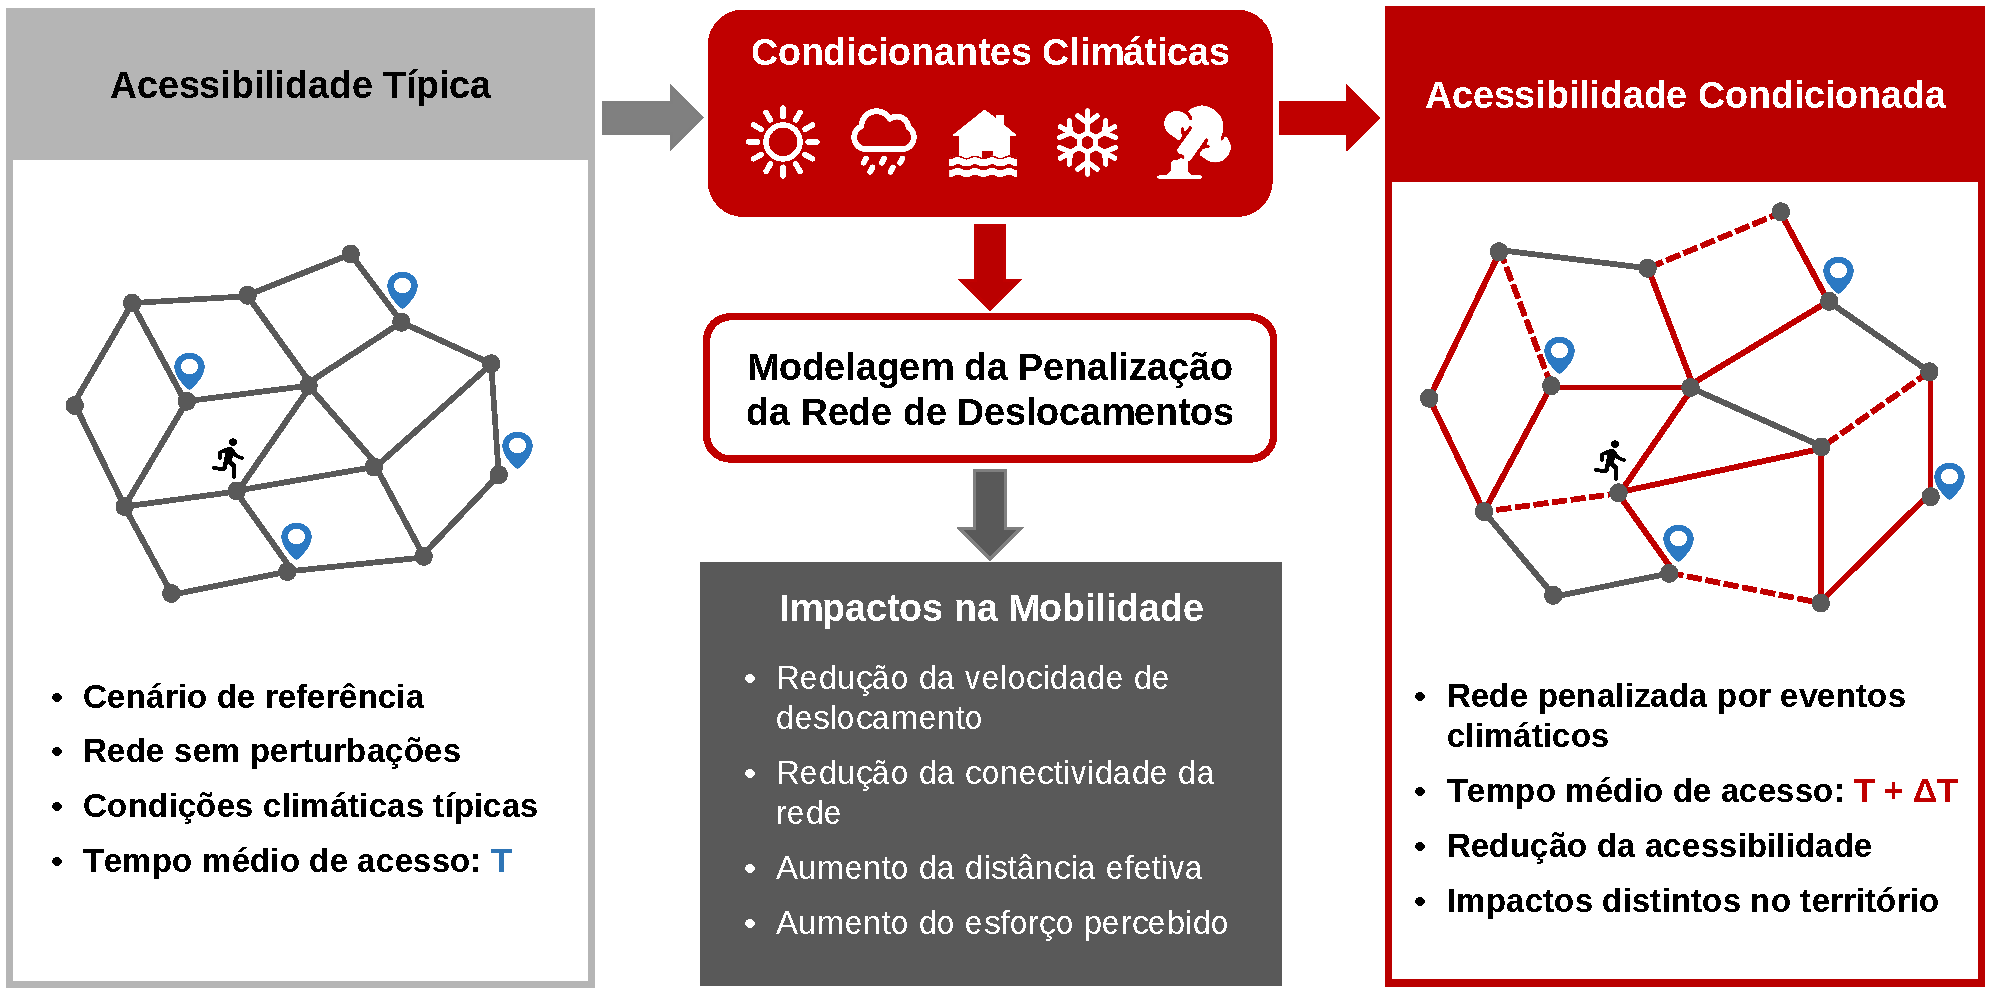
\includegraphics[width=1\textwidth]{figs/framework.pdf}
  \caption{Fluxo de modelagem dos cenários de acessibilidade. À esquerda, a rede no cenário típico, com seus custos originais de deslocamento. Ao centro, o mecanismo de penalização, que utiliza dados ambientais para penalizar a infraestrutura de mobilidade. À direita, o cenário condicionado, no qual o aumento do comprimento das arestas representa visualmente o acréscimo no tempo ou custo de deslocamento provocado pela perturbação.}
  \label{fig:framework}
\end{figure}

% O restante da Seção está estruturado da seguinte forma: a Subseção \ref{subsec:composition} apresenta o processo de coleta, pré-processamento e integração dos dados utilizados na modelagem do território urbano; a Subseção \ref{subsec:processing} descreve o método de cálculo dos indicadores de mobilidade e acessibilidade em diferentes cenários; a Subseção \ref{subsec:comparative} detalha os procedimentos para comparação entre os cenários ideal, típico e condicionado; a Subseção \ref{subsec:socioeconomical} expõe a integração de dados socioeconômicos, permitindo análises de desigualdades de acessibilidade; e, por fim, a Subseção \ref{subsec:case} explica os dados e ferramentas que serão utilizados no estudo de caso para aplicação da metodologia.

\subsection{Modelagem Territorial}
\label{subsec:territorial_modelling}

A modelagem do território urbano consiste na coleta, pré-processamento e integração de cinco camadas de dados espaciais que servem de base para a análise da acessibilidade:

\paragraph{1. Malha de análise:} Uma grade espacial regular que define a unidade mínima de estudo. A resolução da malha é ajustada ao modo de transporte e ao contexto local. O centroide de cada célula funciona como a origem teórica dos deslocamentos, servindo de base para o cálculo e a agregação dos indicadores.

\paragraph{2. Pontos de Interesse (POIs):} Representam os destinos dos deslocamentos. São coordenadas que indicam a localização dos serviços cotidianos da população, organizados em categorias (como saúde, educação e transporte). A seleção depende da disponibilidade de bases de dados locais, sejam oficiais ou colaborativas (crowdsourced).

\paragraph{3. Rede viária:} A infraestrutura de mobilidade é estruturada como um grafo espacial. Os vértices representam os cruzamentos e as arestas representam os segmentos de via, cujo peso base inicial corresponde à distância percorrida. Para possibilitar o cálculo de rotas reais, o centroide de cada célula da malha de análise é vinculado ao vértice mais próximo da rede.

\paragraph{4. Condicionantes ambientais:} Camadas espaciais, que podem ser contínuas (como imagens \textit{raster}) ou discretas (polígonos vetoriais), mapeando os fenômenos climáticos ou ambientais avaliados. Esses dados são sobrepostos à rede viária para reajustar o custo de deslocamento das arestas afetadas no cenário perturbado.

\paragraph{5. Dados Demográficos e Socioeconômicos:} Informações que caracterizam a população residente, como densidade demográfica, renda e escolaridade, oriundas de censos oficiais. Como esses dados são disponibilizados em unidades administrativas irregulares (como setores censitários), aplica-se um procedimento de compatibilização espacial para transferir o perfil socioeconômico para as células da malha regular de análise.

\subsection{Cenários e Perturbações}
\label{subsec:scenarios}

Nesta etapa, a rede de deslocamentos é avaliada em dois estados distintos: (1) Cenário Típico, que reflete as condições normais de mobilidade; e (2) Cenário Condicionado, no qual os custos da rede são alterados por variáveis ambientais.

No \textbf{Cenário Típico}, o peso de cada aresta do grafo ($W_{base}$) corresponde estritamente ao comprimento real do trecho da via. O tempo de percurso em condições normais é obtido dividindo-se essa distância pela velocidade média de deslocamento definida para o modo de transporte analisado.

No \textbf{Cenário Condicionado}, os custos de deslocamento são recalculados por meio de uma função de penalização. Esta função cruza a malha viária com as camadas de condicionantes ambientais ($C$), gerando um peso penalizado ($W_{condicionado}$) para cada aresta, estruturado na forma $W_{condicionado} = f(W_{base}, C)$. A aplicação geométrica dessa função varia conforme a natureza do dado ambiental:

\begin{itemize}
    \item \textbf{Dados contínuos} (ex.: \textit{rasters} de temperatura): O algoritmo extrai a média dos valores dos pixels que se sobrepõem geograficamente à aresta. Esse valor atua como um penalizador contínuo, aumentando o tempo de percurso proporcionalmente à severidade da condição ambiental ao longo daquele trecho.
    
    \item \textbf{Dados discretos} (ex.: polígonos de alagamento ou barreiras físicas): O algoritmo utiliza operações de interseção vetorial. A função pode aplicar multiplicadores severos ou atribuir peso infinito aos trechos interceptados, simulando interdições totais que forçam o roteamento a buscar caminhos alternativos. Essa mesma lógica de interseção pode ser usada de forma inversa, reduzindo pesos para simular áreas favoráveis (como vias arborizadas).
\end{itemize}

A forma matemática da função de penalização $f$ (linear, exponencial, limiar de corte) é um parâmetro ajustável. A escolha e calibração desses parâmetros devem considerar dados ou estudos do contexto local, já que a influência de variáveis ambientais sobre a velocidade e o esforço para caminhar varia conforme o clima, a cultura e as características urbanas. Evidências recentes mostram que fatores como temperatura, clima e condições viárias alteram significativamente o padrão e a velocidade da caminhada \cite{LIANG2020106811,Obuchi2021}. Por isso, recomenda-se que o aplicador utilize valores observados localmente ou reportados na literatura para definir as funções de penalização e os parâmetros do modelo.

Por fim, com os grafos dos dois cenários estruturados, um algoritmo de caminho de menor custo é executado para calcular as matrizes de tempo de viagem. A partir desses tempos, computam-se os indicadores apresentados na Seção \ref{subsubsec:indicadores}: o PTh de cada unidade territorial, o índice G (desigualdade) e o F15 (fração da população atendida) para ambos os cenários.

\subsection{Análise Comparativa}
\label{subsec:comparative}

Nesta etapa, quantificam-se as perdas de acessibilidade comparando diretamente os indicadores do cenário típico com os do cenário condicionado. O objetivo é mensurar a degradação da mobilidade imposta pelos fatores ambientais e identificar pontos críticos onde a dificuldade de circulação provoca maior isolamento.

Essa comparação é estruturada em três procedimentos analíticos principais:

\begin{itemize}
    \item \textbf{Variação relativa:} Cálculo das diferenças absolutas e percentuais dos tempos de deslocamento e dos níveis de acesso entre os dois cenários, evidenciando a magnitude da perda para cada unidade da malha.
    \item \textbf{Validação estatística:} Aplicação de testes de hipótese para confirmar a significância das alterações nos tempos de acesso provocadas pela perturbação ambiental em relação à rede original.
    \item \textbf{Mapeamento espacial:} Uso de métodos de associação local ou clusterização sobre as diferenças de tempo. Isso permite identificar, agrupar e mapear as manchas de degradação, revelando geograficamente as áreas mais penalizadas da cidade.
\end{itemize}

\subsection{Análise de Desigualdade Socioeconômica}
\label{subsec:socioeconomical}

Nesta etapa, as perdas de acessibilidade são analisadas em conjunto com os atributos socioeconômicos da população, com o objetivo de identificar padrões de vulnerabilidade associados às perturbações ambientais.

Cada célula da malha de análise, já associada aos dados sociodemográficos por compatibilização espacial, é tratada como unidade de observação. Para cada célula, consideram-se tanto os indicadores de acessibilidade no cenário típico ($PT_h$) quanto as variações induzidas pela perturbação ($\Delta PT_h$).

Inicialmente, aplica-se um modelo de regressão linear, no qual $PT_h$ e $\Delta PT_h$ são utilizados como variáveis dependentes em especificações distintas. As variáveis independentes incluem renda média, nível de escolaridade, densidade populacional e demais indicadores disponíveis. Esse procedimento permite estimar a associação entre características socioeconômicas e níveis de acessibilidade, bem como sua variação sob condições adversas.

Complementarmente, realiza-se uma análise de agrupamento socio-espacial, na qual as células são agrupadas considerando simultaneamente sua proximidade geográfica e a similaridade em termos de atributos socioeconômicos e indicadores de acessibilidade. Esse procedimento resulta em regiões adjacentes e internamente homogêneas, permitindo identificar padrões territoriais de desigualdade e vulnerabilidade de forma integrada.

% https://geoportal.sgb.gov.br/geosgb/
\subsection{Estudo de Caso}
\label{subsec:case_study}

Para demonstrar a viabilidade da metodologia proposta, o modelo será aplicado em duas capitais brasileiras: Curitiba (PR) e Porto Alegre (RS). A escolha desses municípios permite testar os dois comportamentos da função de penalização definidos na Seção \ref{subsec:scenarios}: o impacto de perturbações ambientais contínuas (temperatura de superfície) e discretas (áreas de risco geológico).

Para garantir a reprodutibilidade da pesquisa, os experimentos priorizam a utilização de dados abertos e bases governamentais oficiais.

\subsubsection{Curitiba: Degradação por Variável Contínua (Clima)}
O experimento em Curitiba avaliará como o desconforto térmico afeta a mobilidade ativa. Neste cenário, a temperatura de superfície atuará como um penalizador contínuo do esforço de deslocamento, aumentando o peso das arestas mais expostas ao calor. Os dados utilizados compreendem:

\begin{itemize}
    \item \textbf{Malha de deslocamento:} Rede viária extraída do OpenStreetMap (OSM), filtrada para infraestrutura caminhável.
    \item \textbf{Pontos de Interesse (POIs):} Coletados via OSM, complementados e validados por bases de alvarás municipais da Prefeitura de Curitiba, categorizados por tipos de serviço.
    \item \textbf{Condicionante ambiental:} Imagens de satélite (\textit{rasters}) do produto \textit{Surface Temperature} obtidas via Earth Explorer (Landsat 8 e 9, sensor TIRS - banda ST\_TRAD).
\end{itemize}

\subsubsection{Porto Alegre: Degradação por Variável Discreta (Risco Físico)}
O experimento em Porto Alegre analisará o impacto de áreas de risco geotécnico e físico sobre a acessibilidade urbana. Como condicionantes ambientais, serão utilizadas camadas vetoriais (polígonos) de \textit{Áreas com Risco a Movimentos de Massa} e \textit{Áreas de Risco Geológico}, ambas disponíveis no portal GeoPOA\footnote{\url{https://gis-smamus.portoalegre.rs.gov.br/dmweb-2-0/}} e resultantes de mapeamento realizado pelo Serviço Geológico do Brasil (SCG/CPRM). Essas áreas atuam como variáveis discretas, simulando barreiras que interrompem ou penalizam rotas afetadas por riscos. Os dados considerados para o experimento são:

\begin{itemize}
    \item \textbf{Malha de deslocamento:} Rede viária extraída do OpenStreetMap (OSM);
    \item \textbf{Pontos de Interesse (POIs):} Serviços e instalações mapeados integralmente a partir do OSM;
    \item \textbf{Condicionantes ambientais:} Polígonos das \textit{Áreas com Risco a Movimentos de Massa} e \textit{Áreas de Risco Geológico} proveniente do GeoPOA (origem: SCG/CPRM).
\end{itemize}

Por fim, para a análise de desigualdade socioeconômica em ambos os municípios, as malhas territoriais serão enriquecidas com dados do Censo Demográfico do IBGE (Instituto Brasileiro de Geografia e Estatística), permitindo o cruzamento das perdas de acessibilidade com variáveis de renda, infraestrutura domiciliar e vulnerabilidade social.

\subsection{Limitações}
\label{subsec:limitations}

A calibração dos efeitos ambientais no modelo é limitada pela disponibilidade e qualidade dos dados ou por falta de estudos específicos. Por isso, os valores de indicadores como o PTh podem não representar tempos absolutos reais, sendo mais adequados para análises comparativas entre diferentes regiões do que para estimativas precisas de tempo. Dessa forma, o modelo cumpre melhor o papel de identificar padrões de desigualdade e vulnerabilidade territorial diante de perturbações ambientais do que de quantificar o tempo exato de acesso.

Além disso, há limitações relacionadas ao comportamento dos indivíduos. Em situações extremas, as pessoas podem optar por não se deslocar ou escolher modos de transporte diferentes da mobilidade ativa. O modelo pressupõe a manutenção do deslocamento a pé mesmo sob condições adversas, o que pode não refletir a realidade observada. Assim, os resultados simulam apenas o impacto potencial das perturbações na acessibilidade da rede, não substituindo análises que considerem efetivamente as escolhas modais dos usuários. Ressalta-se, ainda, que a metodologia pode ser adaptada para outros modos de transporte, mediante ajustes nos parâmetros de velocidade e custo.

Ainda, os indicadores calculados refletem apenas o potencial de acesso espacial e o esforço exigido para atingir determinados destinos, sem considerar fatores como a qualidade, capacidade, funcionamento ou atratividade dos serviços presentes nos POIs. Além disso, esses indicadores não capturam obstáculos subjetivos, como percepção de segurança, conforto ou preferência individual de rotas. Por isso, apesar de úteis para análise territorial comparativa, os resultados não devem ser interpretados como medida direta da experiência do usuário ou garantia de acesso efetivo aos serviços analisados.







\section{Planejamento}

O desenvolvimento desta pesquisa está estruturado nas seguintes etapas, com atividades distribuídas ao longo dos próximos meses, conforme cronograma previsto:

\begin{itemize}
    \item \textbf{Etapa 1: Preparação de Dados}
    \begin{itemize}
        \item \textbf{Junho}: Coleta, pré-processamento e integração dos dados espaciais (redes, POIs, condicionantes ambientais e socioeconômicos).
    \end{itemize}
    
    \item \textbf{Etapa 2: Implementação Computacional}
    \begin{itemize}
        \item \textbf{Julho}: Desenvolvimento dos scripts para aplicação das funções de penalização e cálculo dos indicadores de acessibilidade;
        \item \textbf{Julho}: Parametrização e testes dos algoritmos de rota e penalização.
    \end{itemize}
    
    \item \textbf{Etapa 3: Aplicação Experimental}
    \begin{itemize}
        \item \textbf{Agosto}: Execução dos experimentos nos estudos de caso (Curitiba e Porto Alegre);
        \item \textbf{Agosto}: Geração de mapas e síntese preliminar dos resultados de acessibilidade.
    \end{itemize}

    \item \textbf{Etapa 4: Análise Socioespacial e Síntese de Resultados}
    \begin{itemize}
        \item \textbf{Setembro}: Aplicação das análises de desigualdade, regressão e clusterização;
        \item \textbf{Setembro}: Interpretação e consolidação dos resultados.
    \end{itemize}
    
    \item \textbf{Etapa 5: Redação e Revisão}
    \begin{itemize}
        \item \textbf{Outubro}: Consolidação da coletânea de artigos para defesa;
    \end{itemize}
\end{itemize}

O cronograma prevê a conclusão de todas as etapas em um horizonte de cinco meses, com possíveis ajustes em função do andamento das etapas experimentais e análises complementares.
\section{Resultados Parciais e Esperados}
\label{sec:resultados}

Esta seção descreve os avanços já realizados na pesquisa, validados por meio de publicação científica, e detalha os resultados finais que se espera alcançar com a aplicação completa da metodologia proposta.

\subsection{Resultados Parciais}
Como prova de conceito da etapa de modelagem territorial e cálculo de indicadores, foi desenvolvido o estudo intitulado \textit{"Fatores Socioeconômicos e Desigualdade na Mobilidade de Curta Distância aos Serviços Urbanos de Curitiba"} \cite{sbbd_estendido}, apresentado no Apêndice~\ref{apendice:fatores_socioeconomicos}. O trabalho, focado em deslocamentos a pé, estruturou a rede viária e os Pontos de Interesse das categorias de alimentação, comércio, cultura, educação, saúde e transporte, e calculou métricas de acessibilidade como o PTh, PTc e F15 para o cenário típico.

Por meio de análise de regressão e clusterização espacial, o estudo cruzou os tempos de acesso com variáveis socioeconômicas. Os resultados mostraram que variáveis como escolaridade, empregabilidade e acesso à infraestrutura básica estão diretamente associadas a melhores tempos de acesso aos serviços urbanos em Curitiba. Áreas com maior concentração de pessoas com mais anos de estudo ou maior frequência ao ensino médio tendem a apresentar tempos de deslocamento mais baixos e acesso facilitado, enquanto regiões marcadas por maior vulnerabilidade social, como presença de jovens fora da escola e do trabalho, precariedade de água e esgoto, e moradias em condições inadequadas, registram deslocamentos mais longos. 

A análise espacial confirmou que os maiores tempos de acesso se concentram nos setores periféricos da cidade, ampliando desigualdades já presentes nos indicadores socioeconômicos. Além disso, o estudo também identificou casos pontuais de territórios (\textit{outliers}) com oferta de serviços acima da média do entorno imediato, assim como áreas mais próximas as regiões centrais em situação de exclusão devido à carência de infraestrutura urbana.

Embora o estudo tenha consolidado a coleta de dados e o cálculo base da acessibilidade, ele apresentou limitações que fundamentam o avanço metodológico desta dissertação. O modelo utilizou uma topologia estática, focando exclusivamente no cenário típico a pé, sem considerar barreiras físicas temporárias, perturbações ambientais ou a qualidade e capacidade de atendimento dos serviços.

\subsection{Resultados Esperados}

Com a aplicação integral da metodologia proposta, espera-se demonstrar de forma quantitativa como perturbações climáticas e ambientais podem degradar significativamente a acessibilidade urbana em comparação ao cenário típico. O trabalho deverá validar o mecanismo de penalização do grafo, mostrando na prática como a introdução de camadas ambientais altera o custo do deslocamento e modifica a topologia funcional da cidade. Os resultados esperados incluem a produção de mapas detalhados, capazes de identificar regiões que, embora tradicionalmente bem servidas de acessibilidade, se tornam isoladas ou apresentam forte degradação sob condições ambientais adversas.

Além disso, a análise irá quantificar os efeitos dessas perturbações sobre diferentes grupos sociais, por meio da aplicação de métricas como o Índice G e o cruzamento com indicadores socioeconômicos. Assim, será possível evidenciar se as perdas de acesso afetam a população de forma homogênea ou se recaem de maneira mais intensa sobre territórios e grupos em situação de vulnerabilidade. Espera-se, portanto, fornecer um panorama analítico robusto que possa subsidiar o planejamento urbano e orientar políticas públicas mais resilientes, considerando não apenas a oferta de oportunidades, mas também as barreiras dinâmicas impostas pelo clima e pelo ambiente ao acesso dos cidadãos.

\bibliographystyle{sbc}
\bibliography{refs}

\newpage
\appendix
\pagestyle{empty}

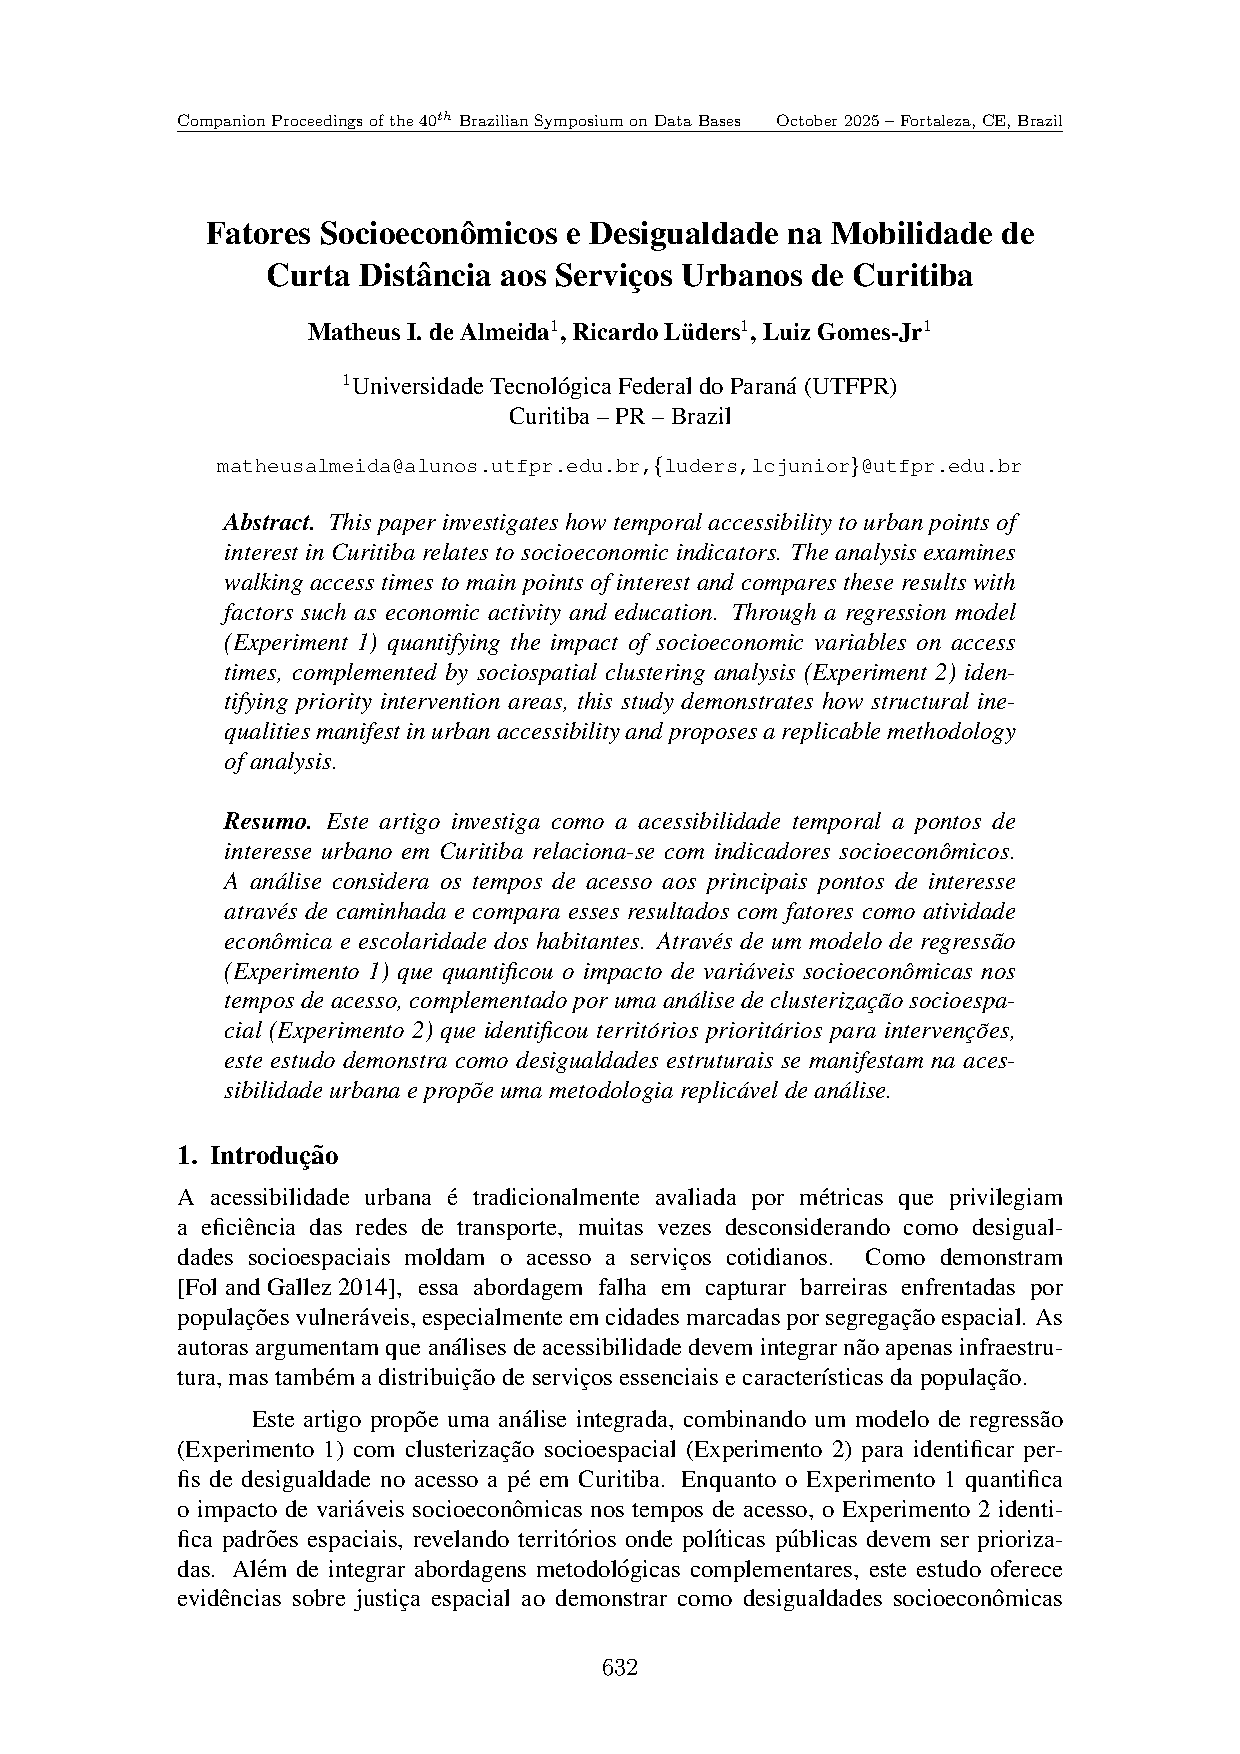
\includepdf[
    pages=1, 
    scale=0.8, 
    pagecommand={\section{Apêndice A}\label{apendice:fatores_socioeconomicos}}
]{files/fatores_socioeconomicos.pdf}

\includepdf[pages=2-, scale=0.9]{files/fatores_socioeconomicos.pdf}

\end{document}
